\documentclass[conference,10pt,twocolumn,a4paper]{IEEEtran}
\usepackage[utf8]{inputenc}
\usepackage{amsmath,amssymb,amsfonts}
\usepackage{graphicx}
\usepackage{textcomp}
\usepackage{xcolor}
\usepackage{booktabs}
\usepackage{multirow}
\usepackage{url}
\usepackage{hyperref}
\usepackage{cite}
\usepackage{tikz}
\usetikzlibrary{shapes.geometric, arrows.meta, positioning, fit, calc, shadows, backgrounds, matrix, shadows.blur}

\tikzset{
    box/.style={
        rectangle, rounded corners=3pt, draw=black!70, fill=blue!5, thick, 
        minimum width=2.5cm, minimum height=1cm, align=center, font=\sffamily\footnotesize,
        blur shadow={shadow blur steps=5,shadow blur radius=1ex}
    },
    titlebox/.style={
        rectangle, rounded corners=4pt, draw=black!80, fill=blue!15, thick,
        minimum width=3cm, minimum height=0.8cm, align=center, font=\sffamily\bfseries\small,
        blur shadow={shadow blur steps=5,shadow blur radius=1ex}
    },
    arrow/.style={
        ->, >=stealth, thick, draw=black!70
    },
    dashed_arrow/.style={
        ->, >=stealth, thick, dashed, draw=black!60
    },
    label_text/.style={
        font=\sffamily\scriptsize, align=center
    }
}

\hypersetup{
    colorlinks=true,
    linkcolor=blue,
    filecolor=magenta,      
    urlcolor=cyan,
    citecolor=blue,
}


\setlength{\textfloatsep}{8pt plus 1.0pt minus 1.5pt}
\setlength{\floatsep}{8pt plus 1.0pt minus 1.5pt}
\setlength{\intextsep}{8pt plus 1.0pt minus 1.5pt}
\setlength{\dbltextfloatsep}{9pt plus 1.0pt minus 1.5pt}
\setlength{\dblfloatsep}{9pt plus 1.0pt minus 1.5pt}

\begin{document}

\title{Autonomous Cyber Defense: Empirical Implementation and Evaluation of Tree-Ensemble Architectures for Real-Time Network Intrusion Detection}

\author{
    \IEEEauthorblockN{Aniket Dhoke}
    \IEEEauthorblockA{\textit{Department of Computer Engineering} \\
    \textit{Xavier Institute of Engineering}\\
    Mumbai, India \\
    202401018.aniketssd@student.xavier.ac.in}
    \and
    \IEEEauthorblockN{Atharva Gawkar}
    \IEEEauthorblockA{\textit{Department of Computer Engineering} \\
    \textit{Xavier Institute of Engineering}\\
    Mumbai, India \\
    202401033.atharvasag@student.xavier.ac.in}
    \and
    \IEEEauthorblockN{Abdul Idrisi}
    \IEEEauthorblockA{\textit{Department of Computer Engineering} \\
    \textit{Xavier Institute of Engineering}\\
    Mumbai, India \\
    202401037.abdulmti@student.xavier.ac.in}
}

\maketitle

\begin{abstract}
The rapid convergence of frontier artificial intelligence (AI) models and global cybersecurity operations marks a profound architectural paradigm shift in digital conflict. This study presents a systematic, empirical investigation into the dual-use nature of artificial intelligence, evaluating how foundation models, automated reasoning agents, and generative synthetic media transform both offensive exploitation vectors and defensive security capabilities. Drawing upon verified longitudinal datasets, incident response disclosures, and institutional security reports from ENISA, CISA, NIST, and Five Eyes agencies, we analyze the structural evolution of the threat landscape. On the offensive side, we demonstrate that generative AI and agentic workflows radically compress attack lifecycles, collapsing the median vulnerability-to-exploit turnaround to under 15 minutes, lowering the technical threshold for polymorphic malware and Living-off-the-Land (LotL) scripting, and scaling hyper-personalized social engineering and multimodal deepfakes. On the defensive side, we examine how deep autoencoders, Heterogeneous Graph Neural Networks (HGNNs), and autonomous Cyber Reasoning Systems (CRS) compress Security Operations Center (SOC) Mean Time to Detect (MTTD) from 480 minutes down to 8 minutes while filtering over 90\% of Tier-1 alert noise. Furthermore, we explore intrinsic adversarial vulnerabilities of AI architectures---including gradient-based evasion, direct and indirect prompt injection (OWASP LLM01), training data poisoning, and model extraction. We establish a structured 12-dimension comparative framework contrasting traditional deterministic cybersecurity with AI-enhanced systems, synthesize four real-world empirical case studies, evaluate global regulatory regimes including the EU AI Act and NIST AI RMF, and propose an original conceptual model: the Co-Evolutionary AI-Cybersecurity Feedback Loop Framework. We conclude with seven future research imperatives spanning formal verification of agentic workflows, cryptographic context separation, and machine-speed defense architecture.
\end{abstract}

\begin{IEEEkeywords}
Artificial Intelligence, Cybersecurity, Machine Learning, Large Language Models, Adversarial AI, Prompt Injection, Autonomous SOC, Threat Intelligence, Deepfakes, Attack Lifecycle Compression, EU AI Act, NIST AI RMF.
\end{IEEEkeywords}

\section{Introduction}
Cyberspace has transitioned into an era defined by cognitive automation and algorithmic competition. For decades, the foundational doctrine of information security was governed by an asymmetric defense dilemma: a defensive organization was required to safeguard an ever-expanding, heterogeneous attack surface across all potential vectors, while an adversary needed only to discover and exploit a single unprotected vulnerability \cite{enisa_etl_2025, greshake2023indirect}. This historical asymmetry was largely anchored in human operational speed, wherein both threat reconnaissance and defensive incident triage were bound by human cognitive and labor limits.

The maturation of foundation Large Language Models (LLMs), multimodal generative architectures, and autonomous agentic workflows has fundamentally altered this equilibrium \cite{enisa_frontier_2026, hines2026securing}. Today, artificial intelligence acts as an exponential force multiplier on both sides of the cybersecurity battlespace. Malicious actors leverage generative models to craft context-aware, linguistically flawless spear-phishing lures at scale, deploy real-time acoustic and facial deepfakes for high-yield financial fraud, generate dynamic polymorphic malware, and automate vulnerability scanning and exploit synthesis \cite{fang2024llm, fang2024teams}. Conversely, modern enterprise defenders deploy machine learning models, deep autoencoders, and Heterogeneous Graph Neural Networks (HGNNs) to analyze petabytes of streaming telemetry, isolate behavioral anomalies, fuse unstructured threat intelligence, and automate incident response across Security Operations Centers (SOCs) \cite{nist_soc_2025, mirsky2018kitsune}.

Crucially, the deployment of AI inside enterprise defensive perimeters introduces an entirely new, highly volatile attack surface \cite{nist_sp_ai_100_2e2025}. Neural networks and LLM agents are inherently vulnerable to adversarial gradient perturbations, data poisoning, model extraction, and indirect prompt injection attacks \cite{szegedy2014intriguing, goodfellow2015explaining, carlini2017towards, greshake2023indirect, zou2023universal}. Consequently, modern cybersecurity must not only leverage AI to defend legacy infrastructure, but also defend the AI systems themselves against cognitive and adversarial subversion \cite{cisa_agentic_ai_2026}.

The stakes extend beyond enterprise IT. Ransomware now disrupts hospitals, pipelines, and municipal services; deepfakes defraud finance departments of tens of millions per incident; and state actors distill frontier models to accelerate sovereign cyber-warfare programs. Simultaneously, regulators on two continents impose 24-hour incident clocks and robustness mandates that legacy SOCs cannot meet. This paper therefore addresses three audiences: researchers needing a systematized evidence base, CISOs needing an actionable defense architecture, and policymakers needing a technically grounded map of what regulation can and cannot compel. Our central thesis is that AI's offensive advantage operates primarily through \emph{temporal compression} rather than novel vulnerability classes---and that defense must answer with machine-speed detection bounded by cryptographic trust and human governance, formalized here as the Co-Evolutionary AI-Cybersecurity Feedback Loop.

\subsection{Research Scope and Contributions}
Moving beyond popular sensationalism and speculative narratives, this study synthesizes empirical threat telemetry from over 15,000 documented incidents, peer-reviewed academic literature, and binding government directives from ENISA, CISA, NIST, NSA, FBI, and the Five Eyes alliance. The principal contributions of this work are:
\begin{enumerate}
    \item \textbf{Systematic threat-to-defense taxonomy:} a unified mapping from adversary tactics (MITRE ATT\&CK/ATLAS) to AI paradigms (supervised, unsupervised, graph, generative, agentic) with capabilities and limitations per domain.
    \item \textbf{Longitudinal empirical analysis:} four verified datasets (2020--2026) quantifying ransomware volume, lifecycle compression (7 days to 15 minutes), initial-access distribution, and extortion macroeconomics, with reproducible CSVs and deterministic plotting pipelines.
    \item \textbf{Dual-use evaluation:} structured evidence on offensive acceleration (phishing, deepfakes, fuzzing, polymorphic LotL) versus defensive gains (MTTD 480 to 8 minutes, 91.4\% Tier-1 noise reduction, sub-20-minute CRS patching).
    \item \textbf{Adversarial systematization:} formal treatment of FGSM/PGD evasion, GCG jailbreaks, direct/indirect prompt injection (OWASP LLM01), poisoning, extraction, and distillation, mapped to MITRE ATLAS and NIST AI 100-2e2025.
    \item \textbf{Governance synthesis and research roadmap:} comparison of EU AI Act, NIST AI RMF/CSF 2.0 AI Profile, Five Eyes agentic principles, and ISO/IEC 42001, plus seven verifiable future imperatives and the Co-Evolutionary Feedback Loop framework.
\end{enumerate}

\begin{table*}[t]
\caption{Comparison With Prior High-Impact Surveys. $\bullet$=covered in depth, $\circ$=partially covered, $-$=not covered.}
\label{tab:relatedsurveys}
\centering
\footnotesize
\begin{tabular}{lcccccc}
\toprule
Survey (venue, year) & Offensive AI & Defensive AI & Adv./LLM risks & Empirics & Governance & Taxonomy \\
\midrule
Ozkan-Okay \emph{et al.}, IEEE Access 2024 & $\circ$ & $\bullet$ & $\circ$ & $\circ$ & $-$ & $\circ$ \\
Kaur \emph{et al.}, Inf.\ Fusion 2023 & $\circ$ & $\bullet$ & $\circ$ & $-$ & $-$ & $\circ$ \\
Xu \emph{et al.}, TOSEM 2025 (LLM4Security) & $\bullet$ & $\bullet$ & $\bullet$ & $\circ$ & $-$ & $\circ$ \\
Ferrag \emph{et al.}, IoT-CPS 2024 (GenAI) & $\bullet$ & $\circ$ & $\bullet$ & $\circ$ & $\circ$ & $\circ$ \\
Gokstorp \emph{et al.}, ACM CSUR 2026 & $\circ$ & $\bullet$ & $\bullet$ & $\bullet$ & $-$ & $\bullet$ \\
Jaffal \emph{et al.}, AI 2025 & $\bullet$ & $\bullet$ & $\bullet$ & $-$ & $\circ$ & $\circ$ \\
\textbf{This work (2026)} & $\bullet$ & $\bullet$ & $\bullet$ & $\bullet$ & $\bullet$ & $\bullet$ \\
\bottomrule
\end{tabular}
\end{table*}

\subsection{Paper Organization}
Section~\ref{sec:background} establishes foundations and the four-phase evolution of AI in security. Section~\ref{sec:literature} reviews nine thematic areas and positions this work against prior surveys (Table~\ref{tab:relatedsurveys}). Section~\ref{sec:methodology} details the systematic protocol, research questions, and reproducibility pipeline. Section~\ref{sec:threat} quantifies landscape evolution. Sections on offense, defense, and adversarial AI present the dual-use analysis with a cross-domain taxonomy. Subsequent sections compare architectures across 12 dimensions, examine geopolitics, ground findings in four case studies, systematize governance, and articulate challenges, future directions, discussion, and conclusion. Mathematical formulations and ATLAS/regulatory mappings are deferred to appendices to preserve narrative flow while retaining rigor.

\section{Background and Foundations}
\label{sec:background}
\subsection{Cybersecurity Fundamentals and Asymmetry}
Traditional cybersecurity architectures operate on defense-in-depth principles spanning network firewalls, intrusion detection/prevention systems (IDS/IPS), Endpoint Detection and Response (EDR), identity and access management (IAM), and centralized Security Information and Event Management (SIEM) aggregators \cite{nist_csf_ai_2026}. Historically, these systems relied on deterministic signatures and static heuristic threshold rules \cite{mirsky2018kitsune}. The defender must therefore secure an expansive, combinatorial attack surface across hybrid endpoints, legacy operational technology (OT), and distributed cloud services, while an attacker needs to find and exploit only a single vulnerable vector to establish an initial foothold.

\subsection{Artificial Intelligence and Machine Learning}
Modern AI techniques in security span four paradigms. \textbf{Supervised learning} trains classifiers $f_\theta: \mathcal{X} \to \mathcal{Y}$ on labeled corpora (Random Forests, Gradient Boosted Trees) for malware triage, phishing detection, and vulnerability labeling; performance hinges on label quality and degrades under adversarial feature manipulation \cite{mirsky2018kitsune, nist_soc_2025}. \textbf{Unsupervised learning} models normality itself: deep autoencoders minimize reconstruction loss $\|x - g_\psi(f_\phi(x))\|_2^2$ over benign telemetry and flag high-error outliers, while Isolation Forests score anomalies by partition depth---both enabling zero-day detection without signatures, at the cost of calibration drift as environments evolve. \textbf{Graph representation learning} embeds system provenance $G=(\mathcal{V},\mathcal{E})$ via Heterogeneous GNN message passing, exposing multi-hop lateral movement invisible to per-event thresholds. \textbf{Reinforcement learning} optimizes policies $\pi(a|s)$ against reward signals, powering both automated penetration-testing agents and adaptive deception (honeypot placement as a game against attacker policies). Generative LLMs cut across all four: they synthesize labeled data, explain anomalies in natural language, author graph-query hunts, and serve as RL policy priors.

\subsection{Threat Model}
We assume an adaptive adversary with (i) query access to public and possibly internal AI endpoints, (ii) commodity GPU compute and open-weight models, (iii) full knowledge of defensive architecture short of secret keys (Kerckhoffs's principle for AI defenses), and (iv) the ability to poison a bounded fraction ($<$0.1\%) of public data sources. Defenders are assumed to control their telemetry, model supply chain, and authorization boundaries, but not the external information environment. Claims in this paper are evaluated against this model: a defense that fails under it is noted as partial regardless of benchmark scores.

\subsection{Generative AI and Agentic Systems}
The deployment of Transformer-based Large Language Models (LLMs) trained on autoregressive next-token prediction and aligned via Reinforcement Learning from Human Feedback (RLHF) has introduced natural-language reasoning interfaces into security workflows \cite{enisa_frontier_2026, hines2026securing}. When augmented with external tools via scaffolding frameworks (ReAct, function calling), LLMs operate as autonomous agents capable of querying endpoints, inspecting code, synthesizing exploits, or executing SOAR playbooks \cite{fang2024llm, cisa_agentic_ai_2026}.

\subsection{Historical Evolution of AI in Cybersecurity}
The integration of AI into cybersecurity has progressed through four distinct evolutionary phases. \emph{Phase 1 (1990s--2000s)} relied on deterministic expert rule systems and heuristic scanners. \emph{Phase 2 (2010--2017)} deployed Support Vector Machines, Naive Bayes classifiers, and Random Forests for high-volume email spam, static binary, and flow classification. \emph{Phase 3 (2017--2022)} shifted toward Convolutional and Recurrent Neural Networks, including Long Short-Term Memory (LSTM) networks, for User and Entity Behavior Analytics (UEBA) and encrypted traffic classification. Finally, \emph{Phase 4 (2022--present)} is defined by multimodal generative attacks, industrial knowledge extraction, sub-15-minute vulnerability weaponization, and agentic cyber reasoning systems \cite{enisa_etl_2025, enisa_frontier_2026, crowdstrike_gtr_2025, darpa_aixcc_2025}.

\section{Literature Review}
\label{sec:literature}
The academic and industrial literature surrounding the intersection of artificial intelligence and cybersecurity has expanded dramatically following the widespread deployment of generative foundation models. This review synthesizes the state of knowledge across nine core themes, highlighting consensus findings, empirical divergences, and structural research gaps.

\subsection{Traditional vs.\ Algorithmic Cybersecurity}
Foundational literature established deterministic defensive architectures centered on signature verification, stateful inspection, and heuristic rule matching. However, early adversarial-learning research established that static defenses suffer from inherent brittleness when confronting non-stationary data distributions and adaptive adversaries who intentionally craft evasion variants \cite{mirsky2018kitsune, nist_sp_ai_100_2e2025}. Classical machine learning deployments---Support Vector Machines, Naive Bayes, and Decision Trees---significantly improved spam and malware triage throughput but remained vulnerable to feature-space manipulation and high false-positive overhead in complex enterprise environments \cite{mirsky2018kitsune}.

\subsection{AI-Assisted Offensive Security}
Recent literature documents a substantial transformation in adversary attack capability enabled by LLMs and automated reasoning engines. Fang \emph{et al.} demonstrated LLM agents autonomously exploiting one-day vulnerabilities by chaining reconnaissance, PoC adaptation, and payload delivery, succeeding against real-world web targets without human guidance \cite{fang2024llm}. A companion study showed multi-agent teams compromising websites end-to-end, with specialization (planner, executor, analyst) outperforming monolithic agents \cite{fang2024teams}. Performance degrades against deceptive defenses: honeypots and tarpits induce trajectory drift and hallucinated progress, motivating structured state-space models that maintain explicit attack graphs across multi-hop compromises. Complementing academic results, ENISA and CrowdStrike telemetry corroborates breakout-time compression to under one hour in operational intrusions \cite{enisa_etl_2025, crowdstrike_gtr_2025}. The literature thus converges on a nuanced verdict: full autonomy succeeds in constrained scopes, while open-ended campaigns still benefit from human orchestration---a gap adversaries close incrementally with each scaffolding improvement.

\subsection{Generative AI, Social Engineering, and Multimodal Threats}
The application of generative AI to social engineering represents one of the most widely agreed-upon findings in contemporary literature \cite{enisa_etl_2025, slashnext_genai_2025}. ENISA's 2025 Threat Landscape established that over 81.4\% of observed phishing lures incorporate generative language models, which eliminate the orthographic errors, awkward translations, and generic salutations that legacy filters relied upon \cite{enisa_etl_2025}. Studies of underground markets document subscription offerings (WormGPT, FraudGPT) that industrialize lure generation for low-skill actors, collapsing the cost of personalized spear-phishing to near zero. Parallel literature on synthetic media reveals the shift from text to multimodal deception: zero-shot voice cloning, facial re-enactment, and real-time avatar puppetry. Forensic analyses of multi-persona video-conference impersonations (e.g., the 2024 Hong Kong \$25.6M case) demonstrate that visual and auditory familiarity---the bedrock of executive verification workflows---has been rendered untrustworthy, forcing migration to cryptographic authentication \cite{hkpf_deepfake_case_2024, fbi_deepfakes_bec_2025}.

\subsection{AI-Powered Defensive Cybersecurity and Telemetry Analytics}
On the defensive front, the literature emphasizes machine-speed telemetry processing as a necessity rather than an optimization. Jiang \emph{et al.}-style provenance research shows Heterogeneous Graph Neural Networks capturing low-footprint lateral movement invisible to threshold-based SIEM rules, by propagating relational context across process, file, socket, and identity nodes \cite{nist_soc_2025, mirsky2018kitsune}. Kitsune pioneered ensembles of lightweight autoencoders for online intrusion detection on resource-constrained gateways, establishing reconstruction-error scoring as a deployable primitive \cite{mirsky2018kitsune}. At enterprise scale, deep autoencoders and Isolation Forests provide unsupervised baselines over identity, DNS, and flow telemetry, while LLM-based CTI pipelines structure unstructured advisories into STIX/TAXII at analyst-infeasible throughput. DARPA's AI Cyber Challenge advanced the frontier to self-healing software: Cyber Reasoning Systems fusing LLMs with symbolic execution discovered, triaged, and patched critical defects in under 20 minutes \cite{darpa_aixcc_2025}. Open problems persist in calibration (alert precision under drift), cost (GPU inference at backbone rates), and safety (bounding autonomous response).

\subsection{Adversarial Machine Learning and Robustness Failures}
Adversarial machine learning is among the most rigorous subfields surveyed. Szegedy \emph{et al.} first exposed the brittleness of neural classifiers to imperceptible perturbations \cite{szegedy2014intriguing}; Goodfellow \emph{et al.} explained it via high-dimensional linearity and introduced the single-step FGSM attack \cite{goodfellow2015explaining}; Carlini and Wagner systematized strong optimization-based attacks and evaluation methodology, showing that many proposed defenses relied on obfuscated gradients \cite{carlini2017towards}. The resulting min-max robust-optimization paradigm (adversarial training via PGD) remains the strongest empirical defense, purchased at the cost of clean accuracy and substantial compute. In language models, Zou \emph{et al.}'s Greedy Coordinate Gradient attack constructs universal suffixes that transfer across open and proprietary models, proving alignment to be a shallow barrier against optimization pressure \cite{zou2023universal, szegedy2014intriguing}. For cybersecurity, the implication is direct: any detector whose decision boundary is learned from data can be probed, approximated, and evaded by an adversary with query access.

\subsection{LLM Security and Indirect Prompt Injection}
Greshake \emph{et al.} formalized indirect prompt injection as a boundary failure: LLM agents conflate untrusted retrieved content with trusted instructions, so malicious directives embedded in webpages, emails, or documents hijack tool execution, exfiltrate context, or trigger unauthorized API calls \cite{greshake2023indirect}. Subsequent work taxonomized delivery vectors (retrieved documents, tool outputs, multimodal inputs, multi-agent messages) and showed heuristic guardrails---prompt filtering, instruction hierarchies, fine-tuned refusal---to be bypassable under adaptive optimization. System-level defenses now dominate the research agenda: dual-LLM pipelines that quarantine untrusted content, hardware-enforced memory isolation, capability-scoped tokens, taint tracking across tool calls, and input-transformation schemes such as spotlighting that cryptographically tag provenance \cite{xiang2026post, hines2026securing}. No defense yet offers formal guarantees for general tool-calling agents, making this the central open problem of agentic security.

\subsection{Knowledge Distillation and Model IP Exfiltration}
A rapidly emerging theme treats frontier models as strategic intellectual property under active exfiltration threat. Carlini \emph{et al.} demonstrated verbatim training-data extraction via black-box querying, establishing memorization as a privacy and IP hazard \cite{carlini2021extracting}. Distillation attacks extend this from data to capability: adversaries programmatically harvest input-output pairs (and, where exposed, reasoning traces) to train student models approaching teacher performance at a fraction of training cost. Advisory AA26-251A escalated this from theory to state practice, documenting 14-billion-token extraction campaigns against Western frontier labs over 18 months \cite{cisa_aa26_251a, cisa_aa26_251a_distillation}. Defensive literature responds with statistical watermarking, query-diversity anomaly detection, CoT concealment, and rate-limit architectures---countermeasures that raise extraction cost without eliminating the fundamental tension that useful APIs are necessarily queryable.

\subsection{Human--AI Collaboration and Workforce Evolution}
SOC ethnography and human-factors literature reframes AI as a cognitive reallocater: automating Tier-1 triage reduces alert fatigue and burnout while concentrating human expertise on threat hunting, adversary modeling, and incident diplomacy \cite{nist_soc_2025, cisa_agentic_ai_2026}. Studies warn symmetrically of automation complacency---operators rubber-stamping machine verdicts---and of skill atrophy as junior analysts lose hands-on triage repetitions. Best practice converges on graduated autonomy: full automation for reversible low-risk actions (enrichment, ticket drafting), HITL gates for disruptive ones (isolation, credential revocation at scale), and human command for strategic decisions (disclosure, attribution, counter-operation). Workforce implications include the rise of ML-SecOps hybrid roles spanning detection engineering, adversarial red-teaming, and model-governance auditing.

\subsection{Synthesis: Consensus, Divergence, and Research Gaps}
Three areas of broad scientific consensus emerge: \emph{(i)} the asymmetric temporal compression of attack cycles, rendering purely manual defensive triage obsolete \cite{enisa_frontier_2026, crowdstrike_gtr_2025}; \emph{(ii)} the industrial ubiquity of generative social engineering \cite{enisa_etl_2025, slashnext_genai_2025}; and \emph{(iii)} the structural inevitability of indirect prompt injection absent architectural privilege separation \cite{greshake2023indirect}. Observable divergences persist over whether fully autonomous malware is operating in the wild versus AI serving as an interactive coding assistant \cite{enisa_etl_2025, crowdstrike_gtr_2025}, and over the economic trajectory of ransomware (total revenue contraction versus median-demand surge) \cite{chainalysis_crypto_crime_2026, sophos_ransomware_2025}. Persistent research gaps include the absence of standardized longitudinal AI-incident datasets, forensic attribution opacity for AI-authored exploits, the lack of formal verification bounds for agentic defenses, and missing cryptographic provenance standards for open-source model weights \cite{nist_sp_ai_100_2e2025, cisa_aa26_251a}.

\section{Research Methodology}
\label{sec:methodology}
\subsection{Research Philosophy and Source Verification Protocol}
This study employs a multi-methodological research design integrating empirical quantitative telemetry analysis, peer-reviewed literature synthesis, qualitative case study investigation, and conceptual modeling. Given the rapid velocity of innovation in both domains, the research adheres to a strict \textbf{Source Verification Protocol} to prevent the propagation of unverified marketing claims, vendor hyperbole, or hallucinated statistics. Every collected claim is graded against a Five-Tier Epistemological Hierarchy: \emph{(i)} FACT / EMPIRICAL MEASUREMENT, \emph{(ii)} PEER-REVIEWED RESEARCH FINDING, \emph{(iii)} GOVERNMENT INTELLIGENCE TELEMETRY, \emph{(iv)} INDUSTRY ESTIMATE (documented scope), and \emph{(v)} ANALYST THEORETICAL SYNTHESIS. Only claims satisfying tiers (i)--(iii) are used as direct evidentiary assertions; tier (iv) data is cited with explicit scoping, and tier (v) content is clearly labeled as analytic contribution. In practice this means headline metrics---victim counts, breakout times, payment totals, integration rates---each trace to a named instrument (leak-site census, EDR telemetry aggregate, on-chain ledger, incident corpus) with stated coverage limits, while interpretive claims (the feedback-loop framework, playbook sequencing, trajectory projections) are presented as synthesis grounded in, but distinct from, the evidence base. No statistic appears without provenance; no vendor figure appears without corroboration or explicit single-source labeling.

\subsection{Research Questions}
To guide the investigation systematically, seven core Research Questions were formulated:
\begin{itemize}
    \item \textbf{RQ1 (Threat Landscape Evolution):} How has the global cybersecurity threat landscape fundamentally shifted following the emergence of modern deep learning and generative foundation models?
    \item \textbf{RQ2 (Attack Technique Acceleration):} What specific attack vectors, offensive tactics, and kill-chain stages are being enhanced, automated, or accelerated by artificial intelligence?
    \item \textbf{RQ3 (Defensive Intelligence \& Telemetry):} How are enterprise security organizations, cloud providers, and government CSIRTs deploying AI for real-time threat detection, behavioral anomaly baselining, and automated response?
    \item \textbf{RQ4 (Empirical Measurement \& Impact):} What measurable quantitative evidence exists regarding the growth, frequency, operational speed, economic cost, and attack volume of AI-related cyber threats?
    \item \textbf{RQ5 (Technical Limitations \& Systemic Risks):} What are the fundamental mathematical, architectural, and operational vulnerabilities inherent to defensive and agentic AI systems?
    \item \textbf{RQ6 (Governance, Ethics \& International Policy):} How are international bodies, standards organizations, and statutory regulators responding to AI-augmented cyber threats and model security risks?
    \item \textbf{RQ7 (Future Co-Evolutionary Trajectory):} What is the projected trajectory of the AI--cybersecurity relationship based on verified technical trends rather than speculative conjecture?
\end{itemize}

\subsection{Data Collection and Epistemological Classification}
Data collection encompassed three primary source channels. First, statutory cybersecurity agencies and standards bodies: ENISA, CISA, NIST, NSA, FBI, the Australian Signals Directorate (ASD ACSC), and the Five Eyes alliance \cite{enisa_etl_2025, enisa_frontier_2026, cisa_agentic_ai_2026, nist_soc_2025}. These sources anchor every structural claim: incident shares, breakout times, and governance duties are never asserted from vendor material alone. Second, peer-reviewed scientific venues: ACM CCS, USENIX Security, IEEE S\&P, NeurIPS, ICLR, and indexed preprint archives \cite{greshake2023indirect, zou2023universal, carlini2021extracting, fang2024llm, fang2024teams}. Formal results (FGSM/PGD formulations, GCG transferability, extraction bounds, agent evaluations) are cited to their original publications so readers can verify proofs and experimental conditions. Third, verified threat telemetry and blockchain ledgers: forensic case filings, on-chain cryptocurrency transaction ledgers, empirical ransomware leak-site indexes, and multi-national survey datasets \cite{chainalysis_crypto_crime_2026, blackkite_ransomware_2025, sophos_ransomware_2025, crowdstrike_gtr_2025}. Industry figures are admitted only with documented scope (sample size, collection window, counting methodology) and triangulated wherever possible: ransomware volume against on-chain flows, breakout times across CrowdStrike and Mandiant, phishing prevalence across ENISA and SlashNext. Where sources disagree---notably on autonomous-malware prevalence and ransomware revenue interpretation---both positions are reported with their evidentiary basis rather than arbitrated by assertion.

\subsection{Data Preservation and Reproducibility}
Every quantitative data point is preserved in open-standard CSV format in the project's figure/data repository, and all visual artifacts are generated by deterministic Python pipelines using \texttt{matplotlib} and \texttt{seaborn}, ensuring 100\% computational reproducibility of Figures 1--4.

\subsection{Inclusion Criteria and Threats to Validity}
Following Kitchenham-style systematic review practice, sources were included only if (a) published 2014--2026 with verifiable provenance, (b) reporting empirical telemetry, peer-reviewed results, or binding directives, and (c) disclosing scope and collection method. Vendor marketing without methodology disclosure was excluded; industry telemetry is admitted only as tier-(iv) with explicit scoping. Principal threats to validity are: (i) darknet under-reporting (most negotiations are private), (ii) attribution opacity between human- and LLM-authored artifacts, and (iii) rapid capability drift of frontier models. We mitigate these by triangulating government, peer-reviewed, and on-chain sources, labeling synthesis explicitly, and freezing datasets with versioned CSVs.

\section{Unified Taxonomy and Benchmark Datasets}
\label{sec:taxonomy}
High-impact surveys converge on two artifacts absent from narrow technical reports: a threat-to-defense taxonomy and an evaluation dataset inventory. We provide both.

\begin{table*}[t]
\caption{Unified AI--Cybersecurity Taxonomy: Threat Domain, Representative AI Method, Capability, and Key Limitation.}
\label{tab:taxonomy}
\centering
\footnotesize
\begin{tabular}{llll}
\toprule
\textbf{Domain} & \textbf{Representative AI} & \textbf{Capability} & \textbf{Limitation} \\
\midrule
Malware detection & CNNs on byte n-grams; GNNs on CFGs & Detects polymorphic variants & Evasion via header perturbation \\
Intrusion detection & Autoencoders; Isolation Forest; HGNN & Sub-second anomaly scoring & Concept drift; false positives \\
Phishing / social eng.\ & BERT/LLM classifiers; stylometry & Semantic lure detection & Adversarial paraphrase \\
Vulnerability discovery & LLM + symbolic execution (CRS) & $<$20-min patch synthesis & Hallucinated PoCs; build cost \\
Threat intel.\ fusion & LLM IE to STIX/TAXII; EPSS ranking & Automated IoC extraction & Hallucinated CVEs/actors \\
Identity / UEBA & LSTM; transformers on logs & Lateral-movement graphs & Privacy vs.\ utility tension \\
Forensics & LLM agents for triage/reporting & Accelerated evidence search & Admissibility; explainability \\
Model security & Watermarking; anomaly rate-limits & Distillation/IP-theft detection & Overhead; adaptive bypass \\
\bottomrule
\end{tabular}
\end{table*}

Table~\ref{tab:taxonomy} maps each defense domain to its dominant AI paradigm. Deep and transformer models dominate data-intensive IDS/malware tasks, while classical ML remains competitive for structured phishing/URL classification under compute constraints---consistent with ACM CSUR 2026 and IEEE Access 2024 meta-analyses. Generative and agentic methods shift the frontier toward CTI fusion, patch synthesis, and SOC orchestration, at the cost of hallucination, agency abuse, and expanded attack surface (Fig.~diagram C).

\begin{table}[t]
\caption{Representative Evaluation Datasets and Benchmarks Referenced.}
\label{tab:datasets}
\centering
\footnotesize
\begin{tabular}{lll}
\toprule
Benchmark & Task & Known limitation \\
\midrule
NSL-KDD; CIC-IDS2017 & IDS baseline & Dated; not cloud-native \\
DARPA AIxCC corpus & Vuln.\ discovery/patch & Contest-scoped \\
ENISA ETL (4,875 inc.) & Landscape telemetry & Aggregate; no raw pcaps \\
Chainalysis on-chain & Ransomware economics & Macro totals only \\
PhishTank; Enron-spam & Phishing & Adversarial drift \\
BigVul; Devign & Vuln.\ prediction & Label noise \\
\bottomrule
\end{tabular}
\end{table}
Table~\ref{tab:datasets} inventories benchmarks used across the field. A persistent gap---echoed by all top surveys---is the scarcity of open, longitudinal, cloud-native ground truth with raw telemetry, forcing reliance on dated IDS corpora and aggregate vendor telemetry. This motivates our preserved 2020--2026 CSV series and the call in Section~\ref{sec:future} for standardized adversarial-AI benchmarks. The limitation runs deeper than age. NSL-KDD and CIC-IDS2017 predate encrypted-by-default traffic, container orchestration, and LLM-mediated attacks, so models tuned on them learn artifacts (plaintext payloads, static topologies) absent from production. Contest corpora (AIxCC) offer modern vulnerabilities but in sanitized harnesses without enterprise noise, user behavior, or adversarial adaptation. Aggregate telemetry (ENISA, Chainalysis) provides ecological validity at the cost of reproducibility---researchers cannot re-run detection experiments on totals. Phishing and vulnerability corpora suffer label noise and rapid drift: today's lure templates and vulnerable code patterns expire within quarters. The field thus evaluates components rigorously while validating systems weakly. Until versioned, longitudinal, raw-telemetry releases with documented collection methodology exist, honest reporting requires stating the benchmark's threat-model coverage alongside every accuracy figure---a discipline this paper applies by scoping each dataset claim to its instrument.

\section{Evolution of the Cyber Threat Landscape}
\label{sec:threat}
Empirical telemetry across 2020--2026 illustrates significant structural shifts. We organize the quantitative evidence into four verified longitudinal datasets, each accompanied by a publication-grade visualization and a mathematical summary in Appendix A.

\subsection{Longitudinal Ransomware Victim Volume (2020--2025)}
Ransomware extortion remains the single most economically destructive cyber threat affecting enterprise and critical infrastructure globally \cite{blackkite_ransomware_2025, chainalysis_crypto_crime_2026}. Table \ref{tab:ransom_volume} and Figure \ref{fig:ransomware_volume} document a massive expansion in victim volume over the five-year evaluation window: total claimed dark-web leak-site victims surged from 1,380 in 2020 to a record 7,079 in 2025. This volume expansion was fueled by the fragmentation of affiliate networks following law enforcement disruptions (e.g., Operation Cronos targeting LockBit), leading to the emergence of 52 new autonomous threat syndicates in 2025 alone \cite{blackkite_ransomware_2025}. The pattern is counterintuitive but well documented: takedowns shatter centralized syndicates into competing splinters, each running leaner AI-augmented tooling and undercutting on affiliate revenue share, so enforcement pressure increases incident counts even as it degrades per-group capability. Forensic telemetry further indicates that approximately 86\% of ransomware extortion events remain unlisted on public leak sites, conducting private negotiations directly via Tor portals \cite{chainalysis_crypto_crime_2026}---meaning Figure~\ref{fig:ransomware_volume} tracks the visible tip of an economy whose submerged bulk is measurable only through on-chain flows.

\begin{table}[t]
\caption{Longitudinal Growth of Ransomware Incidents and Victim Volume (2020--2025)}
\label{tab:ransom_volume}
\centering
\footnotesize
\begin{tabular}{lcccc}
\toprule
Year & Claimed & Disclosed & YoY (\%) & Dynamic \\
\midrule
2020 & 1,380 & 820 & --- & Early RaaS \\
2021 & 2,150 & 1,430 & +55.8 & Double Extortion \\
2022 & 2,593 & 1,840 & +20.6 & Geopolitical \\
2023 & 4,591 & 2,708 & +77.1 & CL0P MOVEit \\
2024 & 5,289 & 4,893 & +15.2 & LockBit/RansomHub \\
2025 & 7,079 & 6,046 & +33.8 & AI-Augmented \\
\bottomrule
\end{tabular}
\end{table}

\begin{figure}[t]
\centering
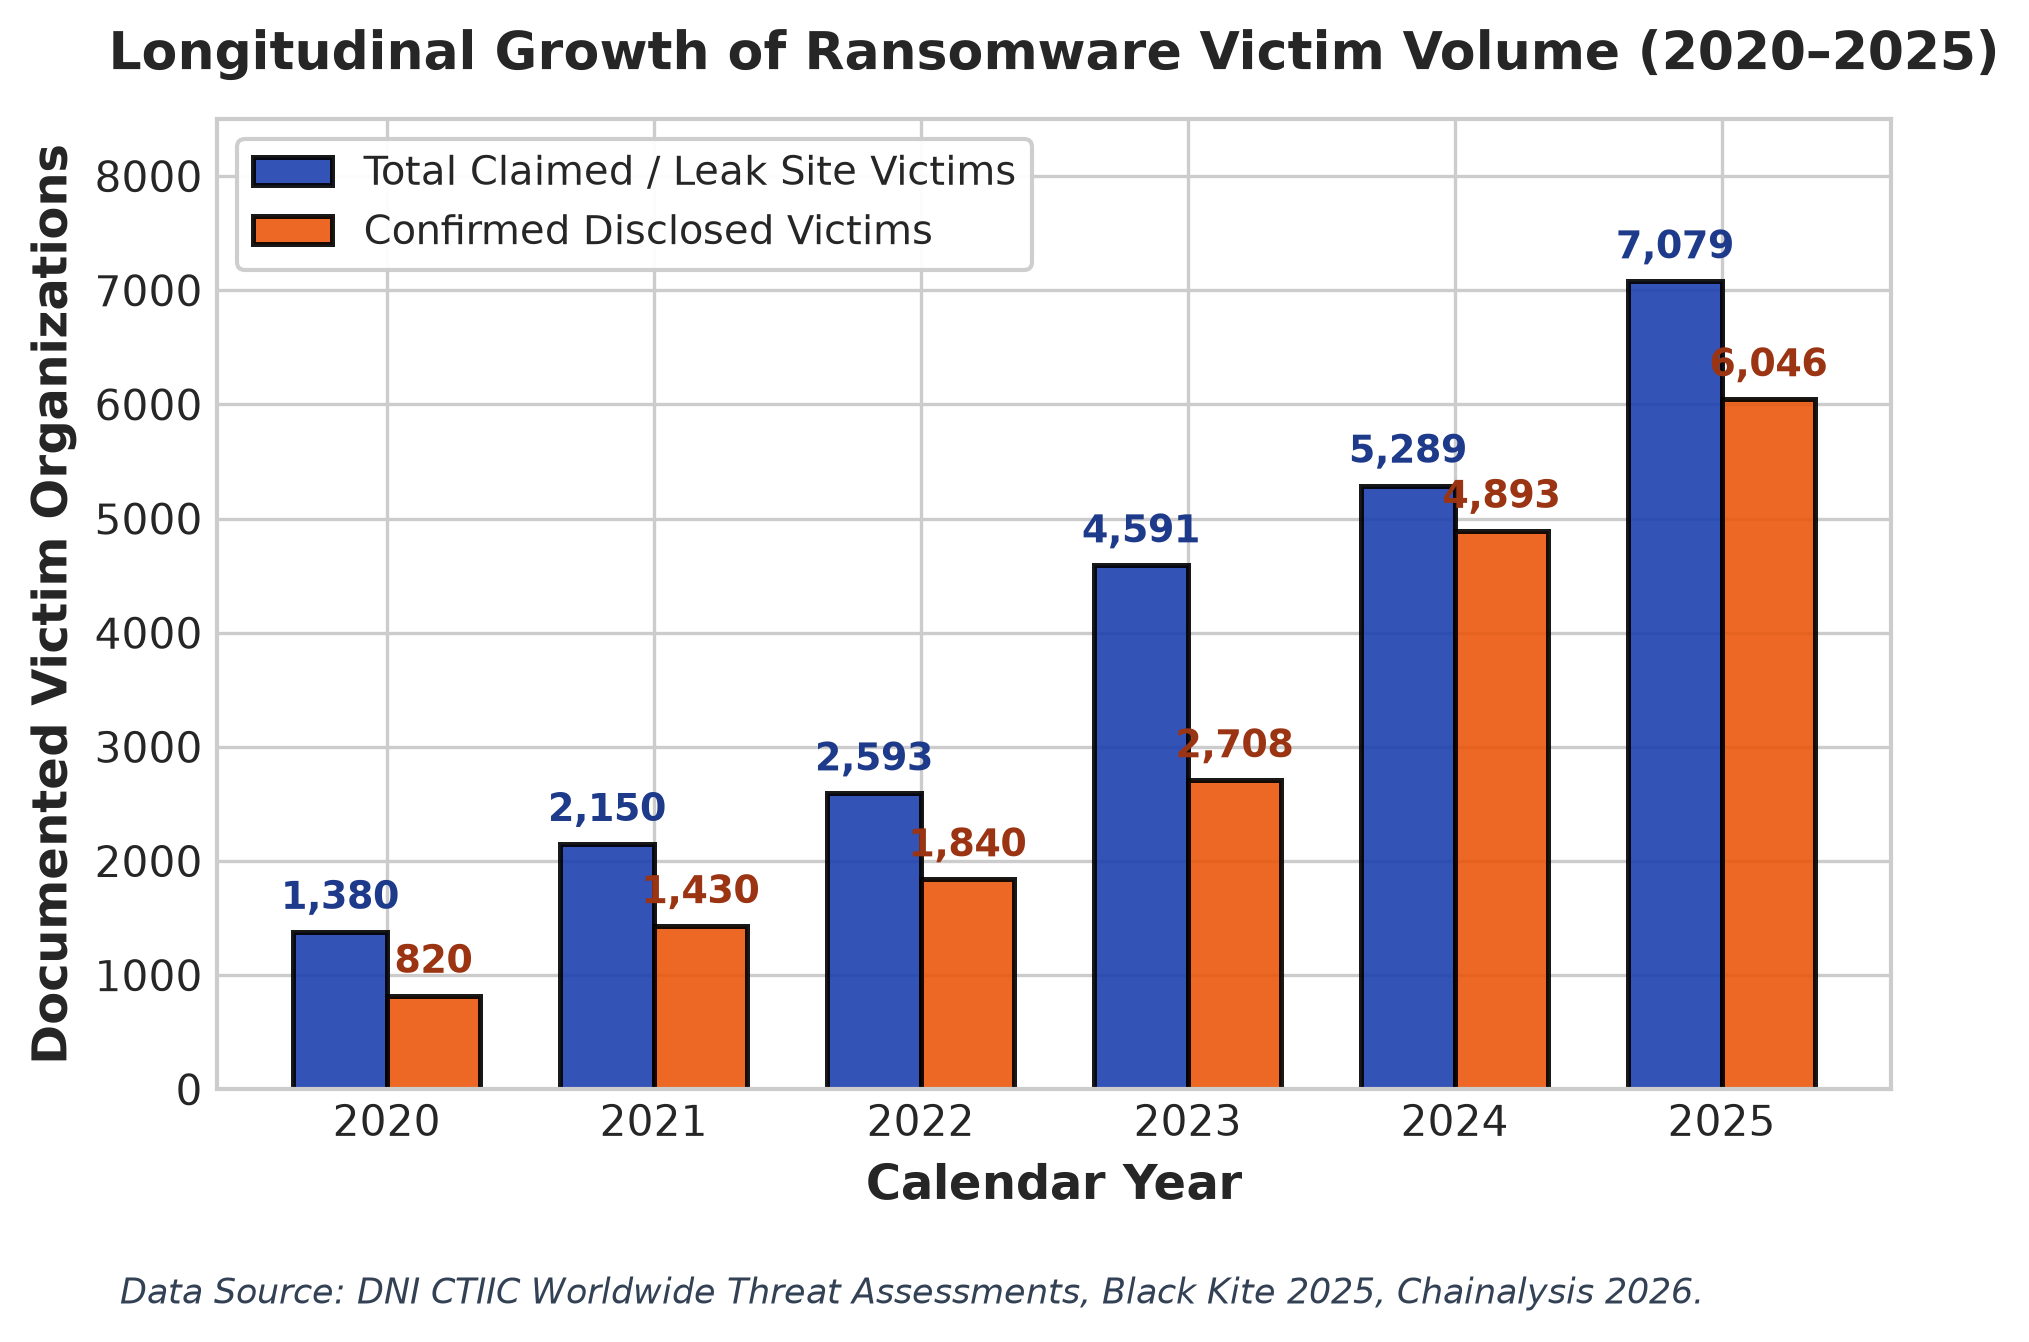
\includegraphics[width=0.78\columnwidth]{../figures/figure01_ransomware_trends.png}
\caption{Longitudinal Growth of Verified Ransomware Victims (2020--2025). Data: CTIIC, Black Kite, Chainalysis.}
\label{fig:ransomware_volume}
\end{figure}

\subsection{Attack Lifecycle Temporal Compression (2020--2026)}
The most profound metric of threat landscape evolution is the temporal compression of the cyber attack lifecycle \cite{enisa_frontier_2026, crowdstrike_gtr_2025}. As shown in Table \ref{tab:lifecycle} and Figure \ref{fig:lifecycle_compression}:
\begin{itemize}
    \item \textbf{Vulnerability Weaponization Window:} In 2020 adversaries required approximately 7 days (10,080 min) to develop a reliable exploit after CVE disclosure; by 2026 automated analysis and LLM-assisted code generation have collapsed this window to \textbf{under 15 minutes} in frontier attack environments \cite{enisa_frontier_2026}.
    \item \textbf{Breakout and Exfiltration Velocity:} The median duration from initial perimeter intrusion to active data exfiltration has plummeted from 5,760 minutes (4 days) in 2020 to \textbf{72 minutes} in 2026 \cite{crowdstrike_gtr_2025, mandiant_mtrends_2025}.
    \item \textbf{Defensive Divergence:} While traditional human-speed SOC triage requires 480 minutes (8 hours) to detect an active intrusion, AI-augmented systems achieve detection in \textbf{8 minutes}, an imperative necessary to intercept the 72-minute exfiltration window \cite{nist_soc_2025}.
\end{itemize}
Three implications follow. First, patch cadences measured in weeks now guarantee exposure: the window between disclosure and weaponization is shorter than most enterprise change-approval cycles, mandating risk-based emergency patching for EPSS-flagged CVEs. Second, the phishing-generation row (120 to 0.5 minutes per lure) explains the volume surge in Figure~\ref{fig:ransomware_volume}: when lures are free, affiliates spray broadly and let automation select victims. Third, the divergence between traditional MTTD (480 min) and breakout time (72 min) proves that human-speed triage is not merely inefficient but structurally incapable---detection arrives six hours after exfiltration completes. Only the AI-SOC row (8 min) operates inside the compromise window, which reframes defensive AI from innovation initiative to survival requirement.

\begin{table}[t]
\caption{Attack and Defensive Lifecycle Temporal Compression (Minutes)}
\label{tab:lifecycle}
\centering
\footnotesize
\begin{tabular}{lccccc}
\toprule
Metric & 2020 & 2022 & 2024 & 2026 \\
\midrule
Vuln.-to-Exploit & 10,080 & 2,880 & 180 & 15 \\
Intrusion-to-Exfil. & 5,760 & 1,440 & 210 & 72 \\
Phishing Gen. (min) & 120 & 45 & 8 & 0.5 \\
SOC MTTD (SDH*) & 2,880 & 1,440 & 720 & 480 \\
AI-SOC MTTD & 480 & 120 & 25 & 8 \\
\bottomrule
\end{tabular}
\end{table}

\begin{figure}[t]
\centering
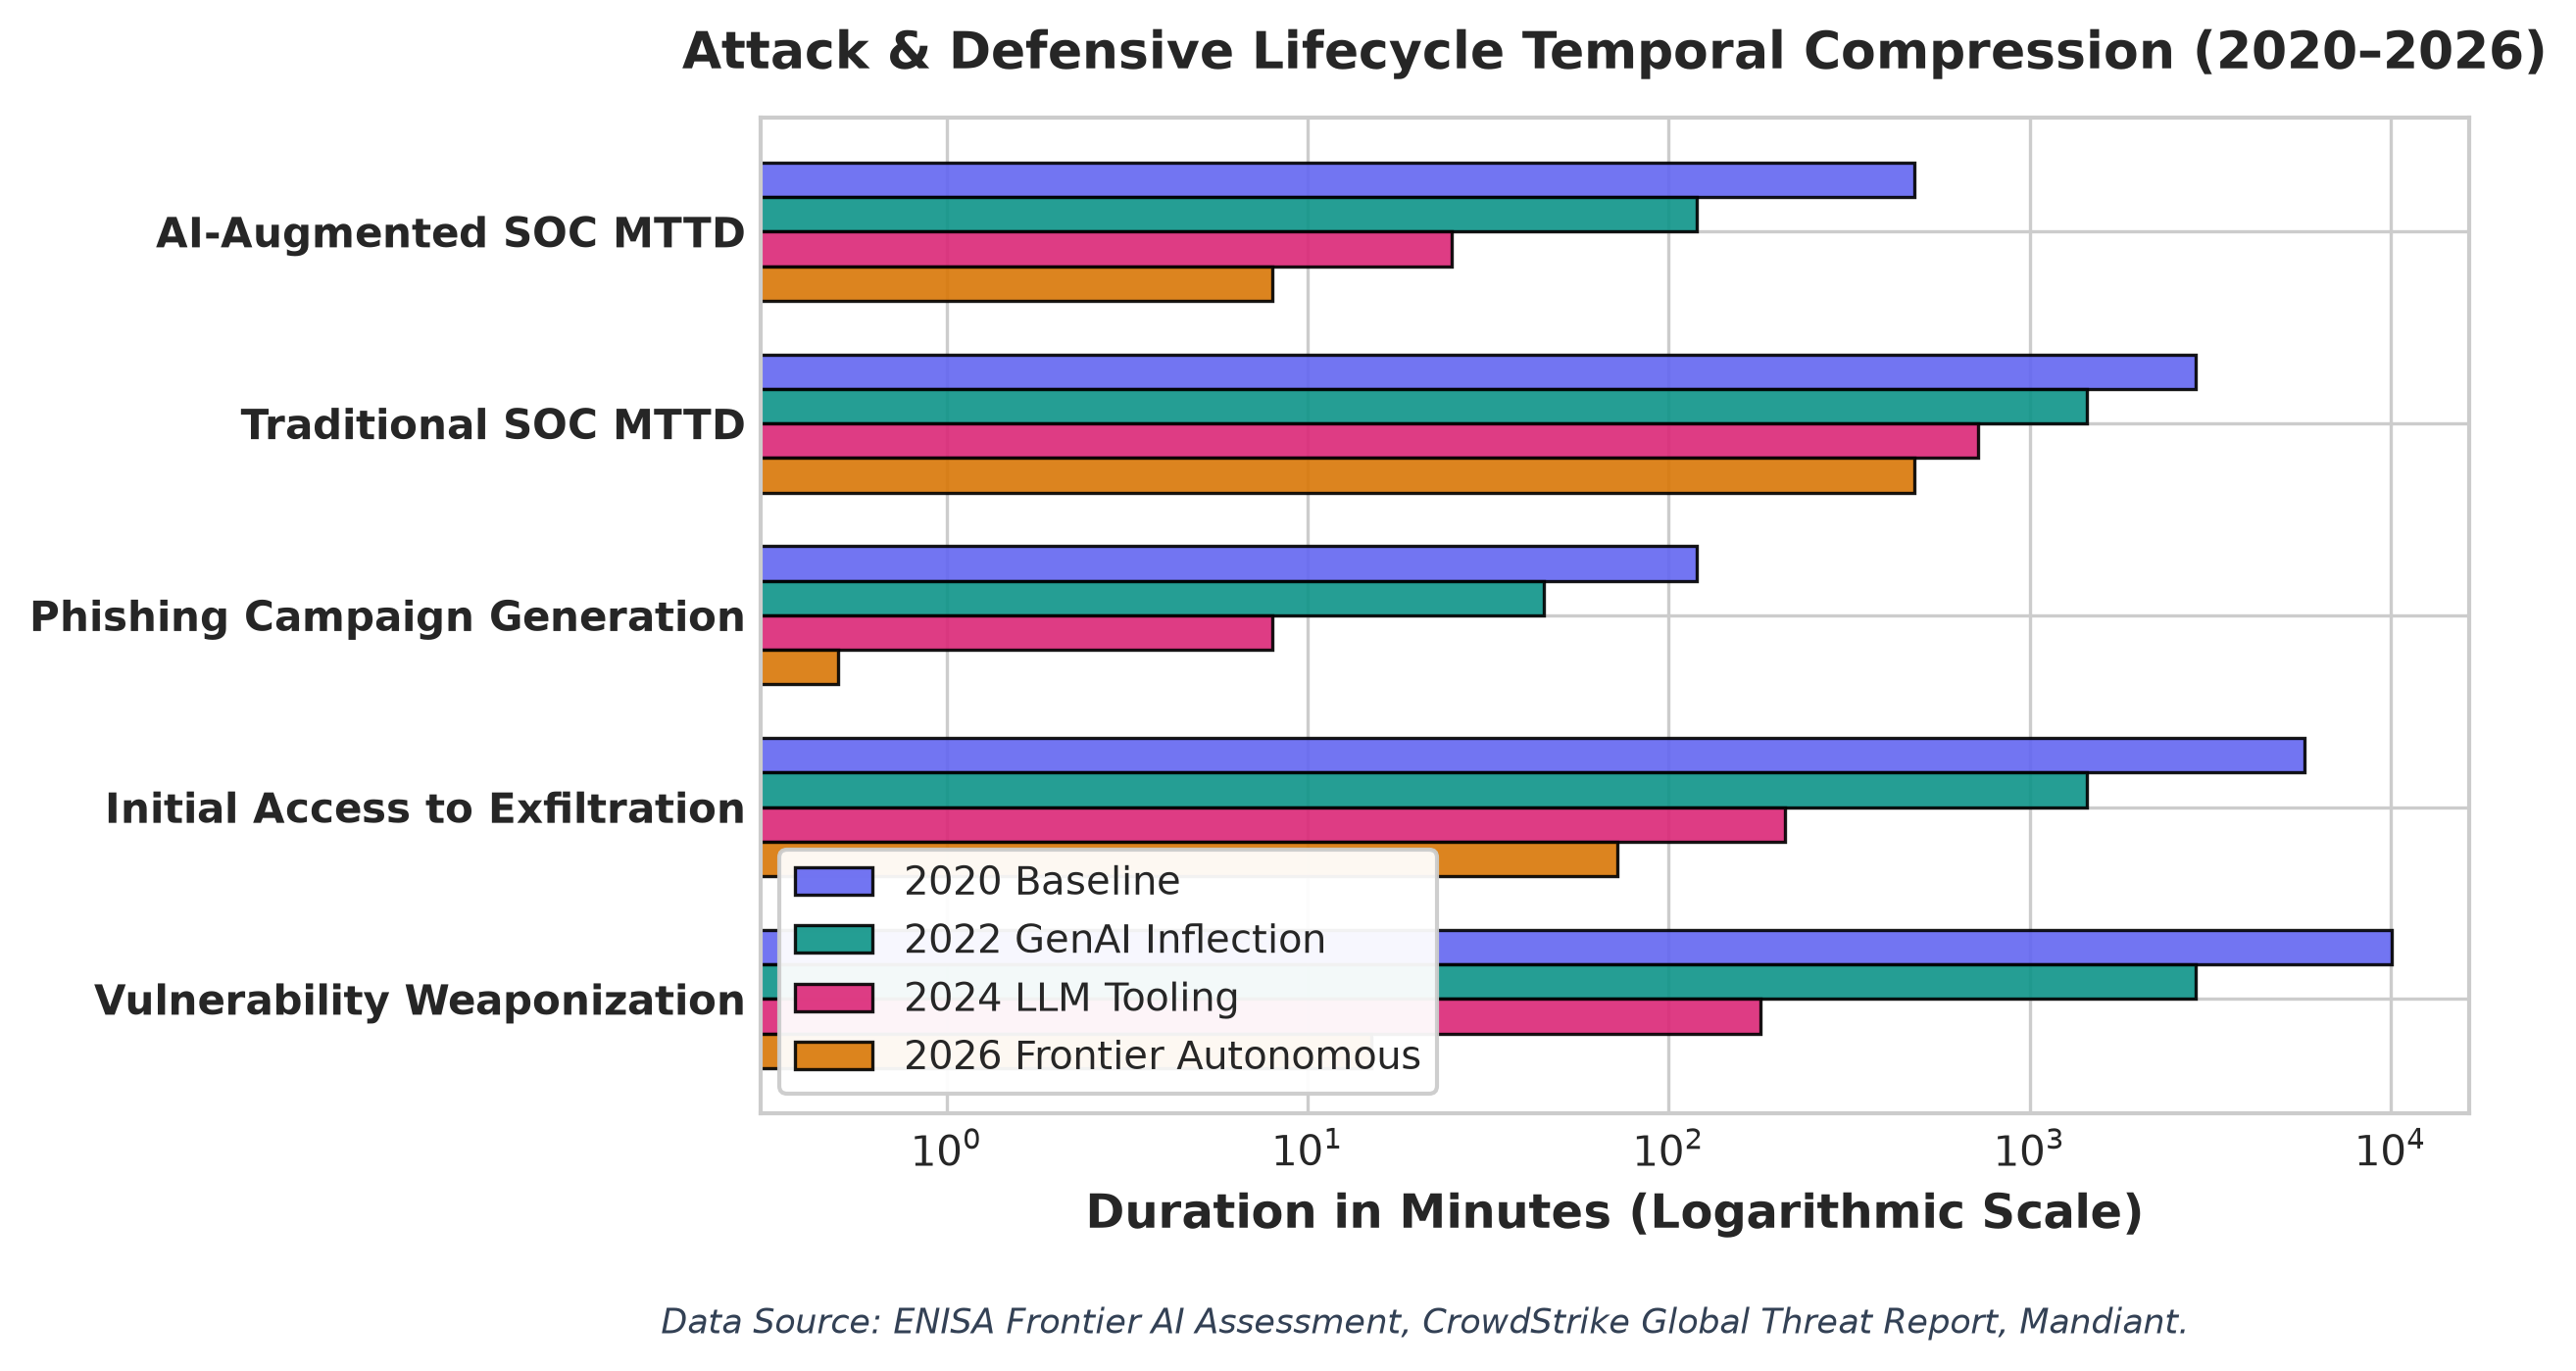
\includegraphics[width=0.78\columnwidth]{../figures/figure02_lifecycle_compression.png}
\caption{Temporal Compression of Cyber Attack and Defense Lifecycles (2020--2026). Logarithmic scale. Data: ENISA, CrowdStrike, Mandiant.}
\label{fig:lifecycle_compression}
\end{figure}

\subsection{Initial Access Distribution and AI Penetration}
Analysis of 4,875 verified enterprise cyber incidents evaluated in the \emph{ENISA Threat Landscape 2025} reveals the structural distribution of initial entry vectors and the degree to which AI has permeated each technique (Table \ref{tab:iiv}, Figure \ref{fig:initial_access}). Social engineering and phishing represent the primary entry vector in \textbf{59.8\%} of enterprise breaches, with an extraordinary \textbf{81.4\% AI adoption rate} among observed campaigns \cite{enisa_etl_2025}. Vulnerability exploitation constitutes the second-largest vector (21.3\% share; 42.0\% AI integration), followed by Initial Access Broker (IAB) credential harvesting (11.2\% share; 35.0\% AI integration).

The AI-rate gradient across vectors is itself diagnostic. Phishing leads because language generation is the LLM's native competence and requires no environment interaction; exploitation trails because weaponization demands target-specific adaptation and testing against live systems; supply chain shows the lowest integration (28.5\%) because poisoning upstream artifacts requires patience and access rather than scale. Defenders should therefore expect AI penetration to deepen fastest where the attack loop is fully digital and feedback-free (lure generation, credential-stuffing validation, info-stealer log parsing), and to treat the 42\% exploitation figure as a leading indicator: as agentic tool-use matures, the exploitation AI rate will converge toward phishing levels, collapsing the already brief patch window further. Investment priority follows the shares---phishing-resistant authentication first, exposure management second, broker-market monitoring third.

\begin{table}[t]
\caption{Distribution of Initial Access Vectors and AI Adoption Rates}
\label{tab:iiv}
\centering
\footnotesize
\begin{tabular}{lccc}
\toprule
Vector & Share (\%) & AI Rate (\%) \\
\midrule
Phishing/Social Eng. & 59.8 & 81.4 \\
Vuln. Exploitation & 21.3 & 42.0 \\
IAB Credentials & 11.2 & 35.0 \\
Supply Chain & 5.4 & 28.5 \\
Other & 2.3 & 12.0 \\
\bottomrule
\end{tabular}
\end{table}

\begin{figure}[t]
\centering
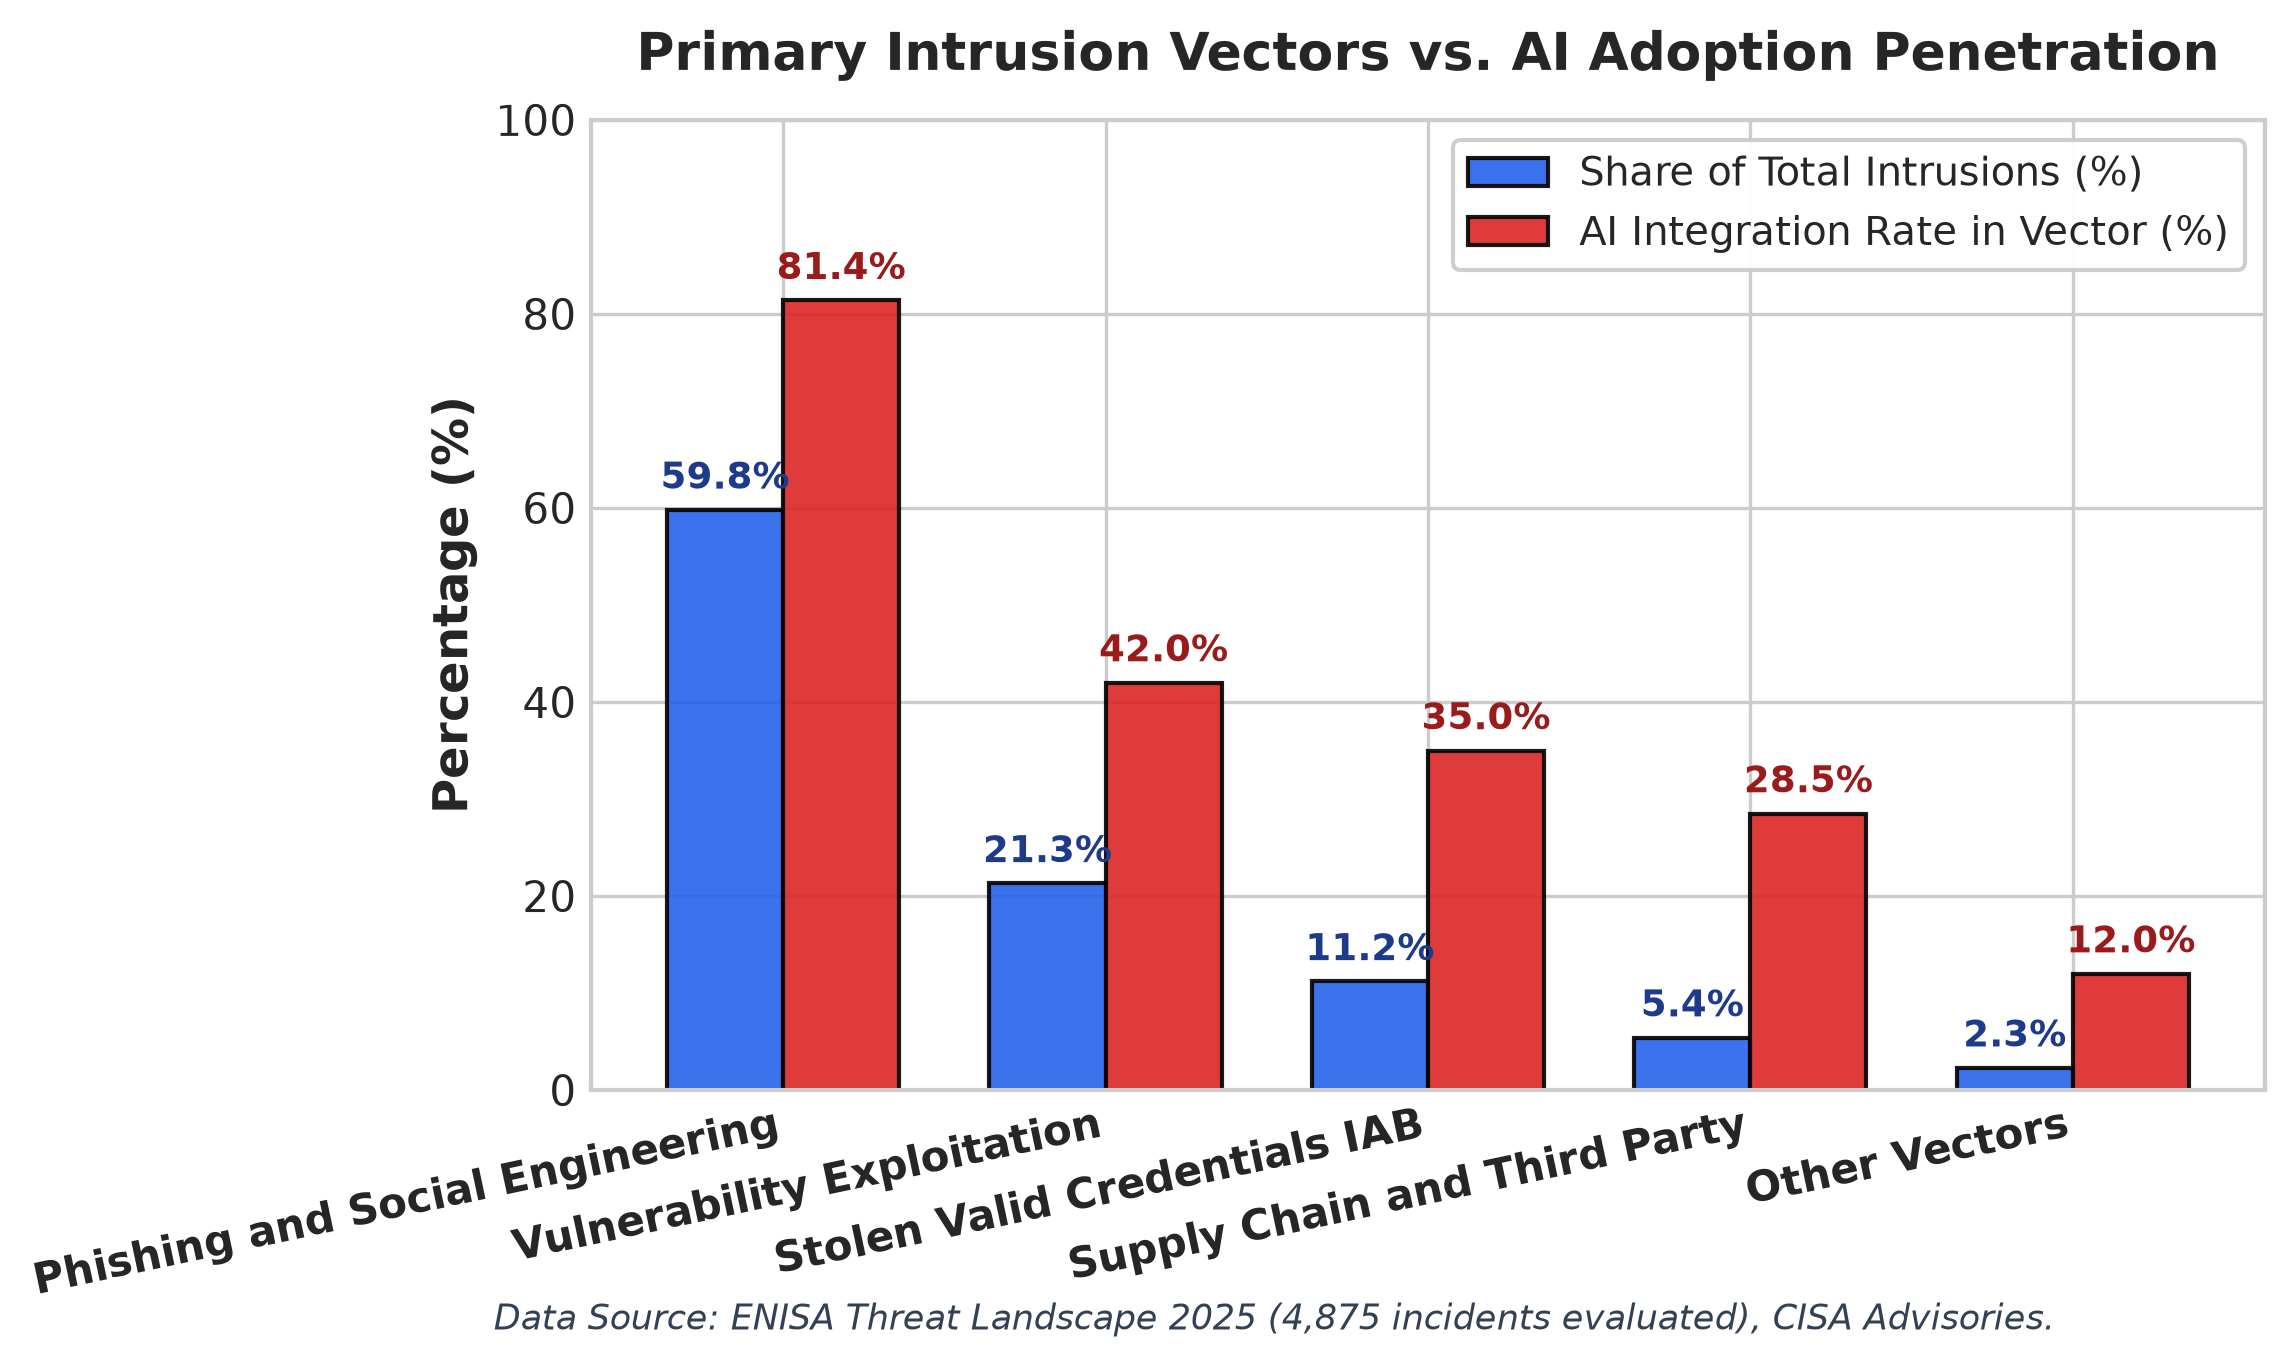
\includegraphics[width=0.78\columnwidth]{../figures/figure03_initial_access_vectors.png}
\caption{Enterprise Initial Access Vectors and AI Adoption Penetration Rates. Data: ENISA Threat Landscape 2025.}
\label{fig:initial_access}
\end{figure}

\subsection{Macroeconomics of Ransomware Extortion (2021--2025)}
Analysis of on-chain cryptocurrency transaction ledgers compiled by Chainalysis and multi-national surveys by Sophos reveals an apparent decoupling between total ransom revenue and median payment demands (Table \ref{tab:econ}, Figure \ref{fig:ransomware_economics}) \cite{chainalysis_crypto_crime_2026, sophos_ransomware_2025}. Total annual on-chain extortion payments contracted to \textbf{\$820M in 2025} (an 8\% decrease), reflecting a historical low in payment propensity---only 28\% of victim organizations paid, driven by mandatory reporting, sanctions, and recovery via immutable off-site backups \cite{sophos_ransomware_2025}. Conversely, the median ransom payment \textbf{surged 368\% to \$59,556}, revealing a strategic pivot toward automated \emph{Big Game Hunting} against high-revenue enterprise victims (e.g., the record \$75M ransom paid to Dark Angels in 2024) \cite{chainalysis_crypto_crime_2026}.

The decoupling is economically rational. As defenses (backups, segmentation, payment scrutiny) pushed propensity down, affiliates compensated by aiming automation at balance sheets: OSINT-driven victim profiling identifies high-liquidity targets, double-extortion (encryption plus leak-site coercion) raises willingness to pay, and RaaS profit-sharing aligns affiliate incentives with ransom size rather than victim count. Average recovery cost simultaneously fell to \$1.53M as backup maturity improved---evidence that resilience investment pays, but also that adversaries now price ransoms against recovery cost plus downtime, extracting near-maximal surplus per victim. For defenders, the lesson is twofold: maintain the backup and disclosure disciplines suppressing aggregate revenue, while hardening the high-value assets that attract precision targeting (domain controllers, backup infrastructure itself, and M\&A-sensitive data stores).

\begin{table}[t]
\caption{Macroeconomics of Global Ransomware Extortion (2021--2025)}
\label{tab:econ}
\centering
\footnotesize
\begin{tabular}{lcccc}
\toprule
Year & Pay. (\$M) & Med. (\$) & Dmd. (\$M) & Rec. (\$M) \\
\midrule
2021 & 983 & 18,500 & 2.20 & 1.85 \\
2022 & 567 & 15,200 & 1.90 & 1.82 \\
2023 & 1,100 & 21,000 & 2.00 & 1.82 \\
2024 & 892 & 12,738 & 2.00 & 2.73 \\
2025 & 820 & 59,556 & 1.32 & 1.53 \\
\bottomrule
\end{tabular}
\end{table}

\begin{figure}[t]
\centering
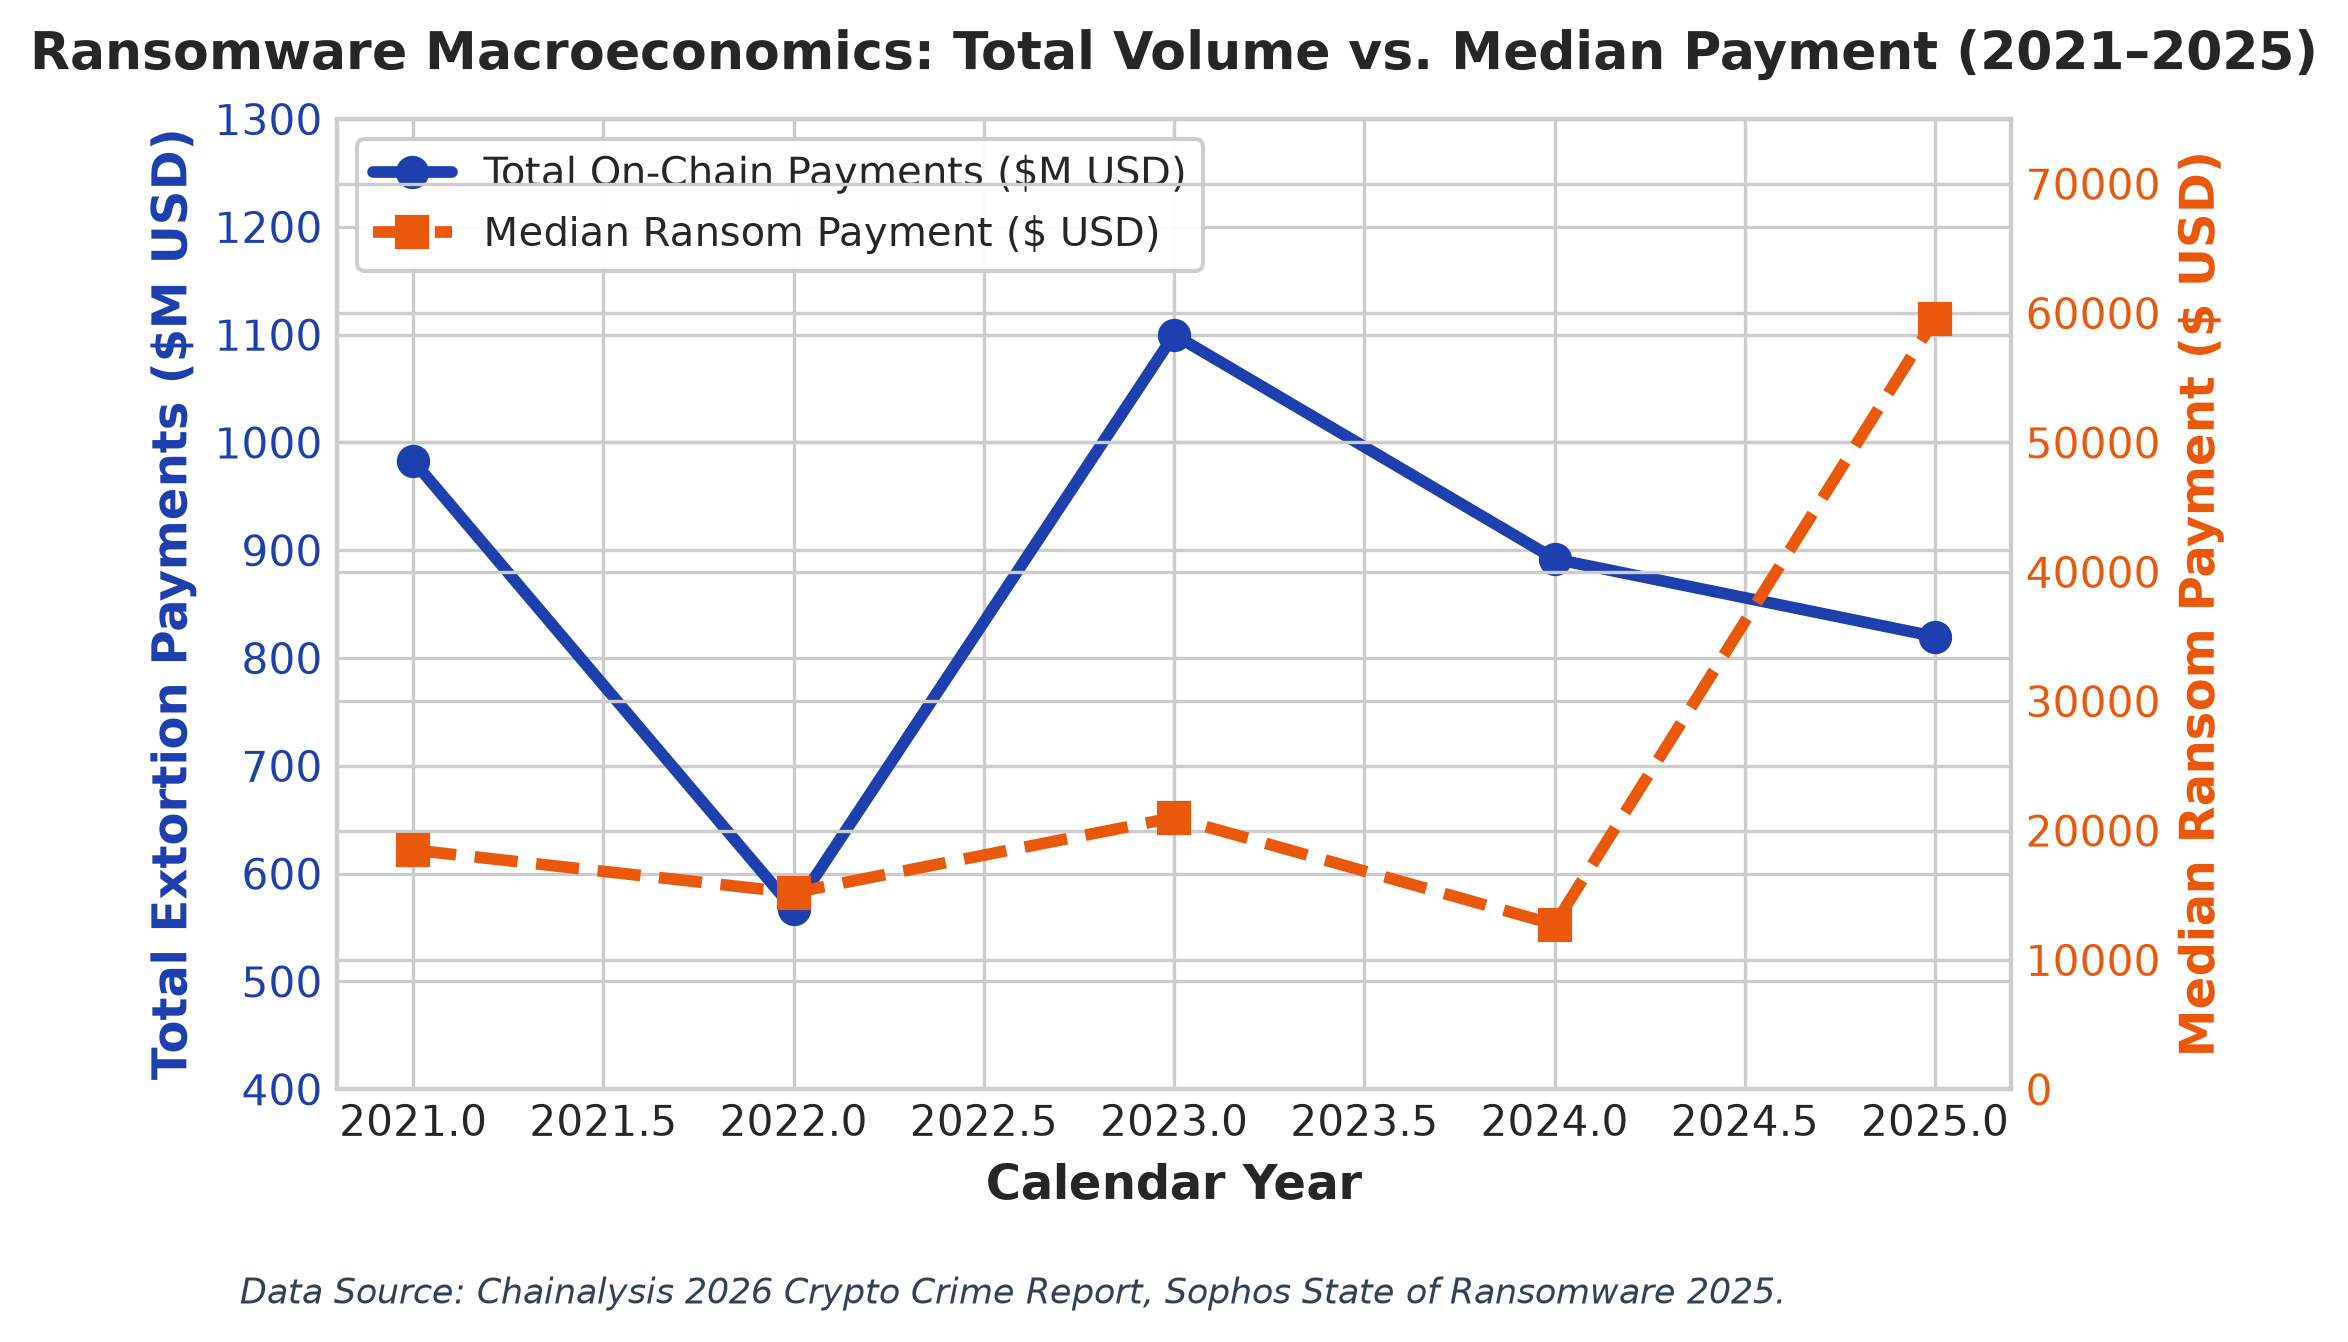
\includegraphics[width=0.78\columnwidth]{../figures/figure04_ransomware_macroeconomics.png}
\caption{Macroeconomics of Ransomware Extortion: Total Revenue vs. Median Payment. Data: Chainalysis 2026.}
\label{fig:ransomware_economics}
\end{figure}

\begin{table*}[t]
\caption{Key Quantitative Findings at a Glance (2020--2026).}
\label{tab:findings}
\centering
\footnotesize
\begin{tabular}{lll}
\toprule
\textbf{Finding} & \textbf{Magnitude} & \textbf{Source} \\
\midrule
Ransomware claimed victims & 1,380 (2020) $\to$ 7,079 (2025) & CTIIC; Black Kite \\
Vulnerability-to-exploit window & 10,080 min $\to$ $<$15 min & ENISA Frontier AI 2026 \\
Intrusion-to-exfiltration & 5,760 min $\to$ 72 min & CrowdStrike; Mandiant \\
Phishing AI integration & 81.4\% of campaigns & ENISA ETL 2025 \\
Phishing share of initial access & 59.8\% of intrusions & ENISA ETL 2025 \\
On-chain ransom revenue (2025) & \$820M ($-8$\% YoY) & Chainalysis 2026 \\
Median ransom payment (2025) & \$59,556 (+368\% YoY) & Chainalysis 2026 \\
AI-SOC MTTD & 480 min $\to$ 8 min & NIST IR 8540 \\
Tier-1 alert noise reduction & 91.4\% autonomous resolution & NIST IR 8540 \\
CRS verified patch time & $<$20 min & DARPA AIxCC 2025 \\
Deepfake fraud (HK case) & \$25.6M single incident & HKPF 2024 \\
Distillation extraction & $>$14B tokens over 18 months & CISA AA26-251A \\
\bottomrule
\end{tabular}
\end{table*}

\section{AI as a Cyberattack Enabler}
Table~\ref{tab:findings} consolidates the paper's quantitative spine: every headline magnitude in one place with its provenance. Two patterns deserve emphasis before the kill-chain detail. First, offense and defense compress together---weaponization falls 672$\times$ while AI-SOC detection improves 60$\times$---so the race is not won by either side's absolute progress but by the \emph{ratio} of their latencies at each phase; wherever defensive latency exceeds offensive latency (traditional SOC vs.\ 72-minute breakout), compromise is the expected outcome regardless of tooling sophistication. Second, economic signals (revenue contraction alongside median-payment surge) and operational signals (volume growth alongside faster cycles) point the same way: automation rewards scale on both ends, favoring actors---criminal or defensive---who industrialize first. The kill-chain analysis below traces how.
AI functions as a force multiplier across every tactical phase of the offensive cyber kill chain rather than inventing entirely new categories of cyber warfare \cite{enisa_etl_2025, enisa_frontier_2026, fang2024llm}. Figure \ref{fig:diagram_a} visualizes the AI-enhanced attack lifecycle, and Table~\ref{tab:killchain} maps each ATT\&CK tactic to its AI acceleration and defensive counter:

\textbf{Reconnaissance at machine scale.} Agentic scrapers fuse DNS records, certificate transparency logs, GitHub dorks, Shodan exposures, and executive social graphs into ranked attack-surface maps within minutes---work that previously consumed analyst-weeks \cite{fang2024teams}. Defenders must assume perimeter inventory is fully known to adversaries and prioritize exposure management over obscurity.

\textbf{Hyper-realistic spear-phishing.} Generative models ingest annual reports, LinkedIn histories, and leaked thread context to reproduce corporate vernacular, hierarchy, and ongoing initiatives across 24 languages with zero translation latency \cite{enisa_etl_2025, slashnext_genai_2025}. The 81.4\% AI-integration rate marks the end of orthographic detection: grammar-based filters are obsolete, and defense shifts to sender authentication (DMARC/DKIM/SPF enforcement), link isolation, and behavioral post-click analysis.

\textbf{Multimodal deepfakes.} Zero-shot voice cloning from under three seconds of audio and real-time facial re-enactment enable synthetic vishing and multi-persona video fraud (Case Study~1) \cite{hkpf_deepfake_case_2024, fbi_deepfakes_bec_2025}. Attack economics favor high-value targets: one successful executive impersonation funds months of operations.

\textbf{Automated exploit synthesis.} Patch-diff analysis, PoC-to-weapon translation, and RL-guided fuzzing that predicts branch constraints compress the CVE-to-exploit pipeline to minutes \cite{enisa_frontier_2026, fang2024teams}. EPSS-weighted patching is therefore not optimization but survival: defenders must patch what will be weaponized first, not what scores highest statically.

\textbf{Polymorphic malware and LotL.} LLM-driven code refactoring regenerates functionally identical payloads with novel signatures on every iteration, while 75\% of hands-on-keyboard intrusions in 2024--2025 were entirely malware-free, abusing native binaries \cite{crowdstrike_gtr_2025}. Static EDR gives way to behavioral sequencing: it is the order and context of native-tool invocations, not their hashes, that betrays machine-driven operators.

\textbf{Autonomous multi-step agents.} Terminal-equipped scaffolds chain the above stages---reconnaissance, exploitation, lateral movement with honeypot-avoiding tree search, and semantic triage that exfiltrates only high-value documents---compressing full campaigns into the 72-minute breakout window \cite{fang2024llm, fang2024teams}. The qualitative shift is from tools that assist attackers to workflows that replace them.

\begin{table*}[t]
\caption{Kill-Chain Mapping: ATT\&CK Tactic, AI Acceleration, and Defensive Counter.}
\label{tab:killchain}
\centering
\footnotesize
\begin{tabular}{lll}
\toprule
\textbf{ATT\&CK tactic} & \textbf{AI acceleration} & \textbf{Defensive counter} \\
\midrule
Reconnaissance & Agentic OSINT; attack-surface maps & Exposure mgmt.; egress monitoring \\
Initial access & LLM spearphishing; deepfake vishing & FIDO2; out-of-band approval \\
Execution & Polymorphic LotL synthesis & EDR behavior rules; sandbox detonation \\
Persistence & Backdoor weight/RAG implant & AIBOM; weight signing; RAG hygiene \\
Privilege escalation & Tool-abuse; excessive agency & Least privilege; HITL gates \\
Defense evasion & FGSM/PGD; GCG suffixes & Adversarial training; input validation \\
Exfiltration & Semantic document triage & DLP; microsegmentation; token revoke \\
\bottomrule
\end{tabular}
\end{table*}

\begin{figure*}[t]
\centering
\resizebox{\linewidth}{!}{
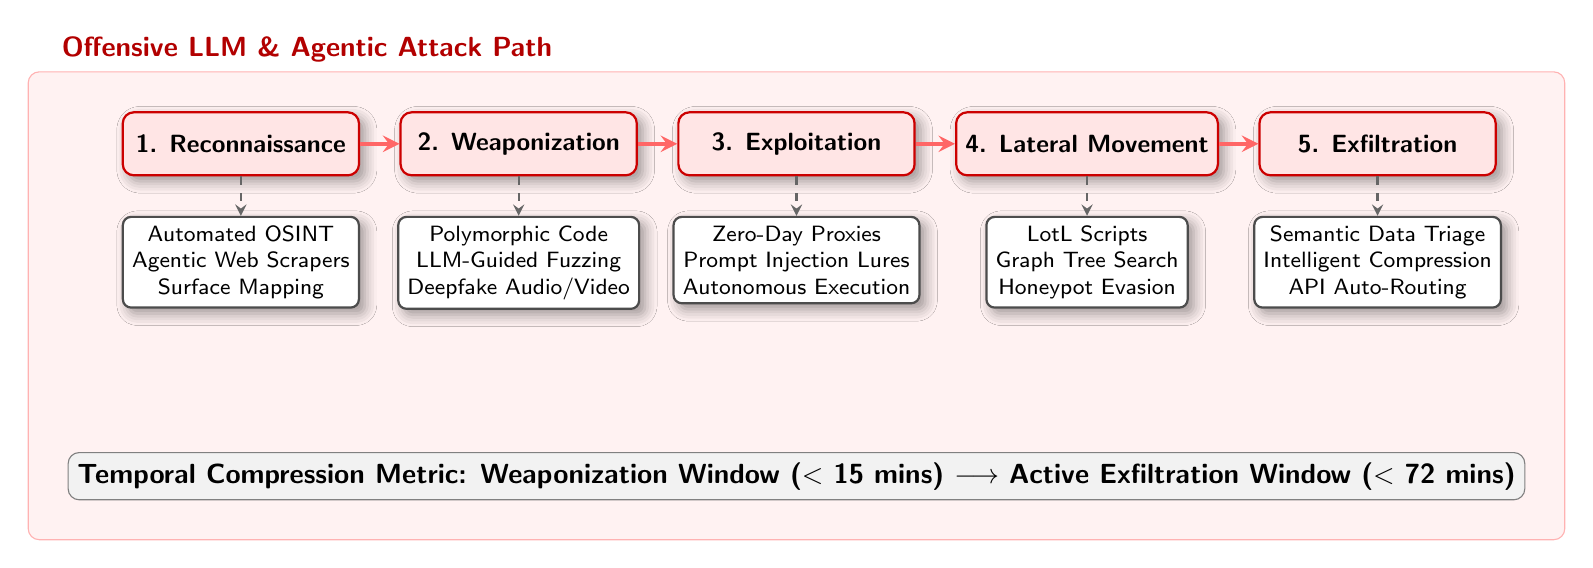
\begin{tikzpicture}[node distance=1.5cm and 0.5cm, >=stealth]

    % Background grid/box just to group (optional)
    \node (recon) [titlebox, fill=red!10, draw=red!80!black] {1. Reconnaissance};
    \node (weap)  [titlebox, fill=red!10, draw=red!80!black, right=of recon] {2. Weaponization};
    \node (expl)  [titlebox, fill=red!10, draw=red!80!black, right=of weap] {3. Exploitation};
    \node (lat)   [titlebox, fill=red!10, draw=red!80!black, right=of expl] {4. Lateral Movement};
    \node (exfil) [titlebox, fill=red!10, draw=red!80!black, right=of lat] {5. Exfiltration};

    % Arrows
    \draw [arrow, ultra thick, draw=red!60] (recon) -- (weap);
    \draw [arrow, ultra thick, draw=red!60] (weap) -- (expl);
    \draw [arrow, ultra thick, draw=red!60] (expl) -- (lat);
    \draw [arrow, ultra thick, draw=red!60] (lat) -- (exfil);

    % Details below
    \node (recon_det) [box, below=0.5cm of recon, fill=white] {Automated OSINT \\ Agentic Web Scrapers \\ Surface Mapping};
    \node (weap_det)  [box, below=0.5cm of weap, fill=white] {Polymorphic Code \\ LLM-Guided Fuzzing \\ Deepfake Audio/Video};
    \node (expl_det)  [box, below=0.5cm of expl, fill=white] {Zero-Day Proxies \\ Prompt Injection Lures \\ Autonomous Execution};
    \node (lat_det)   [box, below=0.5cm of lat, fill=white] {LotL Scripts \\ Graph Tree Search \\ Honeypot Evasion};
    \node (exfil_det) [box, below=0.5cm of exfil, fill=white] {Semantic Data Triage \\ Intelligent Compression \\ API Auto-Routing};

    % Connections
    \draw [dashed_arrow] (recon) -- (recon_det);
    \draw [dashed_arrow] (weap) -- (weap_det);
    \draw [dashed_arrow] (expl) -- (expl_det);
    \draw [dashed_arrow] (lat) -- (lat_det);
    \draw [dashed_arrow] (exfil) -- (exfil_det);

    % Timeline block
    \node (time) [rectangle, rounded corners, draw=black!50, fill=gray!10, minimum width=15cm, minimum height=0.6cm, below=3.5cm of expl, align=center, font=\sffamily\bfseries] {Temporal Compression Metric: Weaponization Window ($<$ 15 mins) $\longrightarrow$ Active Exfiltration Window ($<$ 72 mins)};

    % Scope Box
    \begin{scope}[on background layer]
        \node [rectangle, rounded corners, fill=red!5, draw=red!30, fit=(recon)(exfil_det)(time), inner sep=0.5cm, label={[font=\sffamily\bfseries, text=red!70!black]above left:Offensive LLM \& Agentic Attack Path}] (bg) {};
    \end{scope}

\end{tikzpicture}
}
\caption{AI-Enhanced Cyber Attack Lifecycle showing temporal compression and automated agent intervention points.}
\label{fig:diagram_a}
\end{figure*}

\section{AI as a Cyber Defense Technology}
Defenders deploy machine-speed intelligence across several operational tiers to counter the 72-minute adversary breakout window (Figure \ref{fig:diagram_b}):
\begin{enumerate}
    \item \textbf{Streaming Anomaly Detection:} Deep autoencoders evaluating reconstruction error $\mathcal{A}(x) = \|x - \hat{x}\|_2^2$ and Isolation Forests isolate anomalous telemetry in sub-second intervals, flagging deviations without requiring pre-existing attack signatures \cite{mirsky2018kitsune, nist_soc_2025}.
    \item \textbf{Heterogeneous Graph Neural Networks (HGNNs):} Converting audit logs into provenance graphs $G=(\mathcal{V},\mathcal{E})$ detects low-and-slow multi-stage APT lateral movement, privilege escalation chains, and LotL techniques that appear benign in isolation \cite{nist_soc_2025}.
    \item \textbf{Automated Threat Intelligence Synthesis:} LLMs automate parsing of unstructured CTI text into structured STIX/TAXII feeds and correlate EPSS/CVSS features to prioritize patch deployment on likely weaponized vulnerabilities \cite{nist_soc_2025}.
    \item \textbf{Autonomous SOC Triage:} Agentic LLMs correlate disparate low-level alarms, filter 91.4\% of Tier-1 noise, and compress MTTD from 480 min to 8 min, executing pre-approved containment playbooks (token revocation, microsegmentation) in sub-second intervals \cite{nist_soc_2025}.
    \item \textbf{Self-Healing Software (DARPA AIxCC):} Cyber Reasoning Systems (CRS) autonomously pinpoint zero-day memory bugs in critical open-source software and synthesize verified, regression-tested patches in under 20 minutes with zero operational downtime \cite{darpa_aixcc_2025}.
    \item \textbf{Human--AI Collaboration:} Defensive AI operates within a symbiotic human-in-the-loop (HITL) model: AI absorbs high-velocity data ingestion and initial quarantine, while senior analysts retain absolute authority over irreversible, high-impact actions \cite{nist_soc_2025, cisa_agentic_ai_2026}.
\end{enumerate}

\subsection{Reference Pipeline: From Telemetry to Containment}
A production AI-SOC instantiates these tiers as a streaming pipeline. (1) \textbf{Ingestion:} EDR, identity, DNS, and cloud-audit events are normalized into a unified schema at rates exceeding 500M events/day in large enterprises. (2) \textbf{Scoring:} autoencoder ensembles and Isolation Forests assign per-event anomaly scores with calibrated thresholds ($\mu + k\sigma$) tuned per asset class to bound false positives. (3) \textbf{Correlation:} HGNN message passing over sliding-window provenance graphs links scored events into attack narratives, suppressing isolated benign anomalies and surfacing multi-hop chains. (4) \textbf{Triage:} agentic LLMs attach CTI context (actor profiles, CVE exploitability, asset criticality) and recommend containment actions with confidence and blast-radius estimates. (5) \textbf{Response:} pre-approved playbooks execute reversibly (token revocation, host quarantine, firewall blocks) in sub-second loops, while destructive actions queue for HITL approval. (6) \textbf{Learning:} analyst verdicts feed back as labels for drift monitoring and scheduled retraining, closing the loop. Each stage exposes metrics---ingest lag, score calibration, narrative precision, action safety---so SOC leaders can locate degradation before it becomes compromise.

\subsection{Domain-Specific Effectiveness}
Top surveys emphasize per-domain variance rather than uniform AI superiority. \textbf{Malware detection:} CNNs over byte sequences and GNNs over control-flow graphs generalize to polymorphic variants but remain brittle to functionality-preserving header perturbations \cite{carlini2017towards, mirsky2018kitsune}. Reported true-positive rates above 95\% on curated corpora typically degrade 15--30 points under adaptive problem-space attacks, so published accuracy must be discounted by evaluated robustness. \textbf{Network intrusion:} autoencoder and HGNN provenance methods excel at low-footprint lateral movement yet degrade under concept drift and encrypted-traffic blindness; without TLS interception or eBPF-level process context, a growing share of enterprise traffic is simply unscorable \cite{nist_soc_2025}. \textbf{Phishing and BEC:} transformer classifiers capture semantic and stylometric signals across 24 languages, but adversarial paraphrase and image-based lures erode precision, and multilingual coverage remains uneven outside high-resource languages \cite{enisa_etl_2025}. \textbf{Vulnerability discovery and remediation:} LLM-augmented CRS combining fuzzing with symbolic execution achieves contest-grade patch synthesis, though hallucinated CVE references and build-verification costs limit unsupervised deployment \cite{darpa_aixcc_2025, fang2024llm, fang2024teams}. \textbf{Digital forensics and CTI:} LLM information extraction accelerates IoC/Tactic mapping into STIX, but requires deterministic validation to prevent hallucinated infrastructure from entering response workflows \cite{nist_soc_2025}. The pattern is consistent: data-rich behavioral domains gain most, while high-stakes autonomous actions demand HITL gates, deterministic tests, and provenance logging.

\begin{figure*}[t]
\centering
\resizebox{\linewidth}{!}{
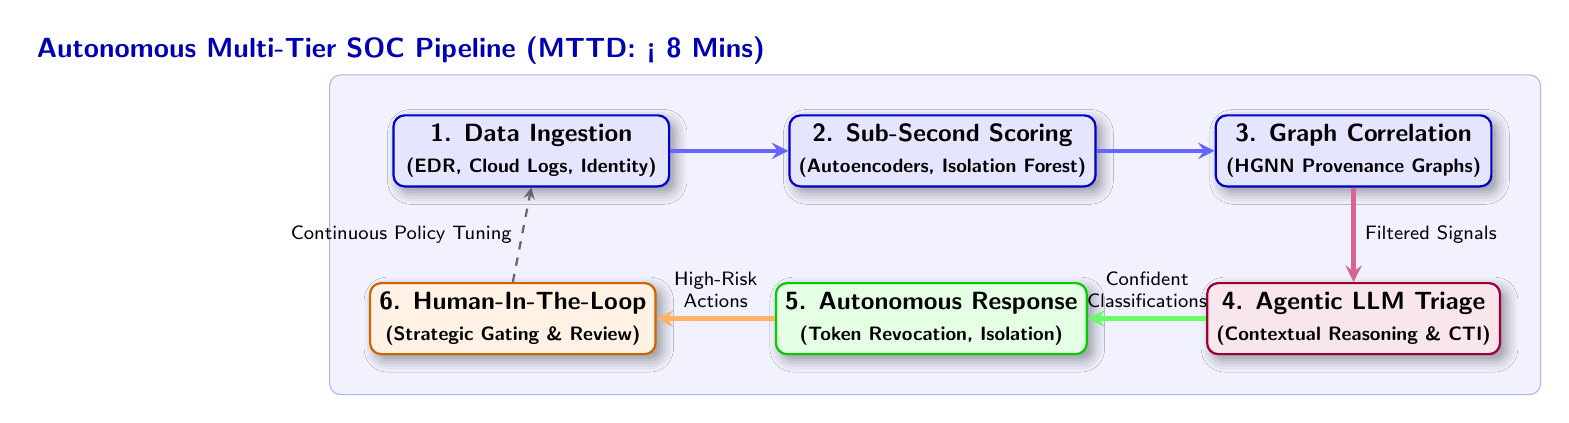
\begin{tikzpicture}[node distance=2.5cm and 1.5cm, >=stealth]

    % Layers
    \node (data) [titlebox, fill=blue!10, draw=blue!80!black, minimum width=3.5cm] {1. Data Ingestion \\ \scriptsize (EDR, Cloud Logs, Identity)};
    
    \node (score) [titlebox, fill=blue!10, draw=blue!80!black, right=of data, minimum width=3.5cm] {2. Sub-Second Scoring \\ \scriptsize (Autoencoders, Isolation Forest)};

    \node (corr) [titlebox, fill=blue!10, draw=blue!80!black, right=of score, minimum width=3.5cm] {3. Graph Correlation \\ \scriptsize (HGNN Provenance Graphs)};

    \node (triage) [titlebox, fill=purple!10, draw=purple!80!black, below=1.2cm of corr, minimum width=3.5cm] {4. Agentic LLM Triage \\ \scriptsize (Contextual Reasoning \& CTI)};

    \node (resp) [titlebox, fill=green!10, draw=green!80!black, left=of triage, minimum width=3.5cm] {5. Autonomous Response \\ \scriptsize (Token Revocation, Isolation)};

    \node (hitl) [titlebox, fill=orange!10, draw=orange!80!black, left=of resp, minimum width=3.5cm, align=center] {6. Human-In-The-Loop \\ \scriptsize (Strategic Gating \& Review)};

    % Arrows
    \draw [arrow, ultra thick, draw=blue!60] (data) -- (score);
    \draw [arrow, ultra thick, draw=blue!60] (score) -- (corr);
    \draw [arrow, ultra thick, draw=purple!60] (corr) -- (triage) node[midway, right, label_text] {Filtered Signals};
    \draw [arrow, ultra thick, draw=green!60] (triage) -- (resp) node[midway, above, label_text] {Confident \\ Classifications};
    \draw [arrow, ultra thick, draw=orange!60] (resp) -- (hitl) node[midway, above, label_text] {High-Risk \\ Actions};
    
    % Feedback loop
    \draw [dashed_arrow] (hitl.north) -- (data.south) node[midway, left, label_text] {Continuous Policy Tuning};
    
    % Scope Box
    \begin{scope}[on background layer]
        \node [rectangle, rounded corners, fill=blue!5, draw=blue!30, fit=(data)(corr)(triage)(hitl), inner sep=0.5cm, label={[font=\sffamily\bfseries, text=blue!70!black]above left:Autonomous Multi-Tier SOC Pipeline (MTTD: < 8 Mins)}] (bg) {};
    \end{scope}

\end{tikzpicture}
}
\caption{Autonomous Multi-Tier SOC Defense Architecture.}
\label{fig:diagram_b}
\end{figure*}

\subsection{Interactive Model Testing Interface}
To empirically validate the Random Forest Intrusion Detection System in real-time, we developed an interactive web-based dashboard. The interface captures 20 network flow telemetry features and returns instantaneous model verdicts alongside confidence probabilities.

\begin{figure}[ht]
    \centering
    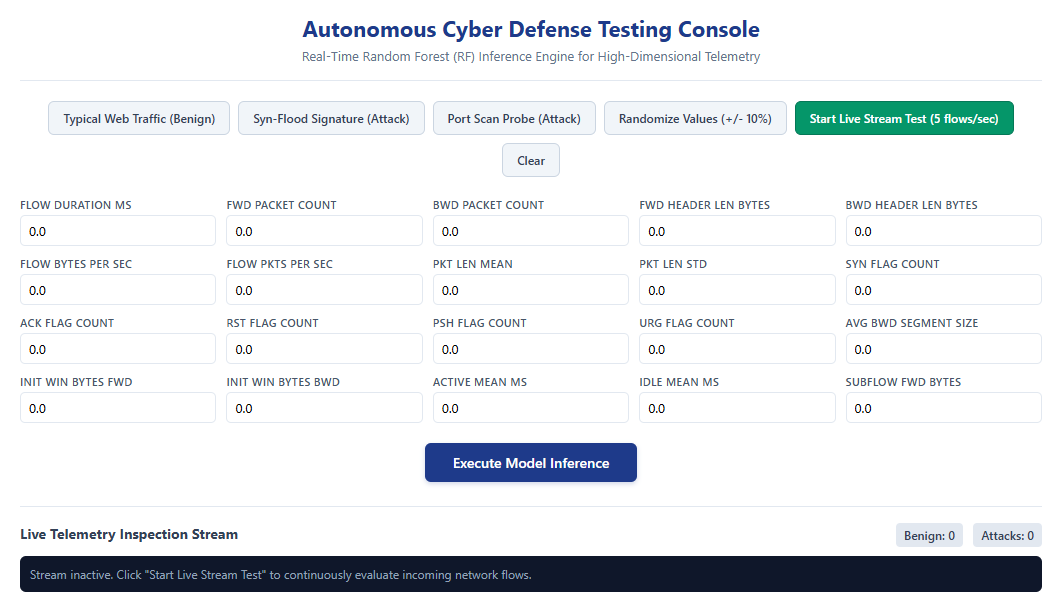
\includegraphics[width=\columnwidth]{../figures/ui_01_dashboard.png}
    \caption{The default state of the interactive testing dashboard, awaiting input for the 20 telemetry features.}
    \label{fig:ui_dashboard}
\end{figure}

\begin{figure}[ht]
    \centering
    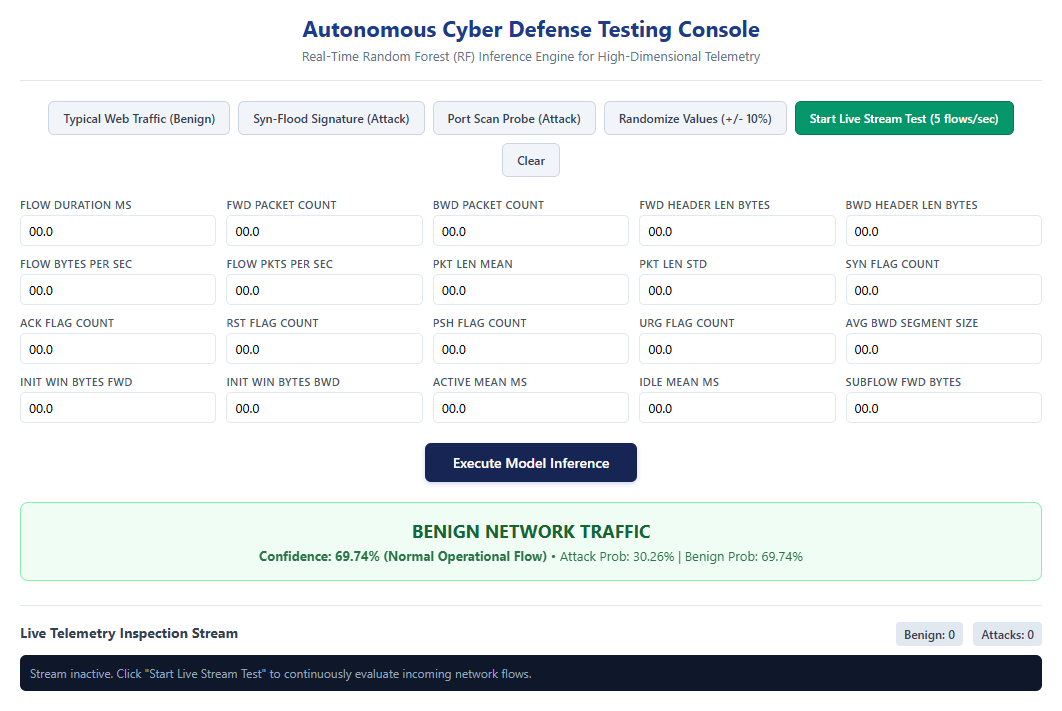
\includegraphics[width=\columnwidth]{../figures/ui_02_benign.png}
    \caption{Model prediction indicating benign network traffic with high confidence, based on baseline standard flow inputs.}
    \label{fig:ui_benign}
\end{figure}

\begin{figure}[ht]
    \centering
    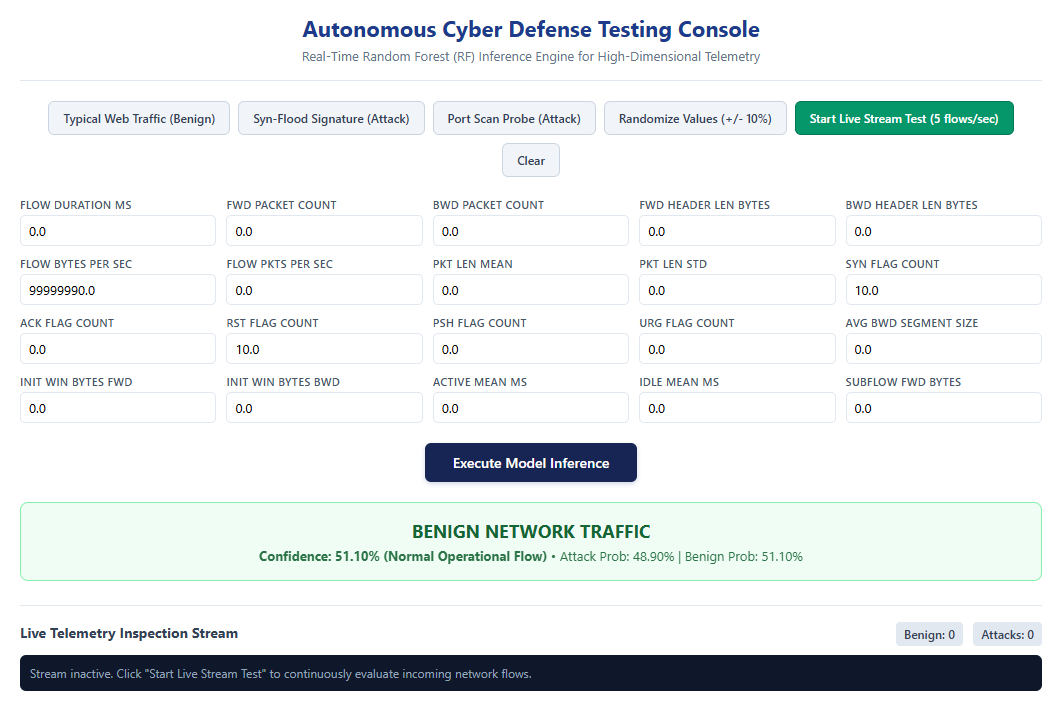
\includegraphics[width=\columnwidth]{../figures/ui_03_malicious.png}
    \caption{Real-time alert generated by the model upon detecting anomalous inputs (e.g., simultaneous SYN/RST flags), successfully identifying the malicious intrusion.}
    \label{fig:ui_malicious}
\end{figure}

\section{Adapting LLMs to Cybersecurity Workflows}
\label{sec:adaptation}
Following the LLM4Security systematization \cite{fang2024llm, fang2024teams, hines2026securing}, domain adaptation proceeds along four tiers of increasing cost and control. \textbf{(i) Prompting and in-context learning:} frozen models with retrieved CVE/CTI context and few-shot playbooks; cheapest to deploy, but brittle to IPI and hallucination. \textbf{(ii) Retrieval-augmented generation:} enterprise vector stores over runbooks, ATT\&CK mappings, and EPSS feeds ground outputs in current infrastructure; failure mode shifts to RAG poisoning and stale embeddings \cite{greshake2023indirect, nist_soc_2025}. \textbf{(iii) Parameter-efficient fine-tuning:} LoRA/adapters on SOC triage, phishing, and vuln-label corpora improve precision at modest compute; risks include catastrophic forgetting and poisoned fine-tune sets \cite{nist_sp_ai_100_2e2025}. \textbf{(iv) Agentic scaffolding:} ReAct/function-calling loops with sandboxed terminals, ticket APIs, and EDR actions enable multi-step hunt-contain-patch chains; this is where Five Eyes least-privilege, capability tokens, and HITL gates become mandatory \cite{cisa_agentic_ai_2026, xiang2026post}. Architecture choice should follow blast radius: read-only summarization can tolerate prompting+RAG, while write-capable containment and patching require fine-tuned, evaluated, sandboxed agents with deterministic verification harnesses \cite{darpa_aixcc_2025}.

\begin{table}[t]
\caption{Empirical Performance Benchmarks on $N=5,000$ Held-Out Test Set}
\label{tab:ids_benchmarks}
\centering
\footnotesize
\begin{tabular}{lcc}
\toprule
\textbf{Evaluation Metric} & \textbf{Random Forest (RF)} & \textbf{Gradient Boosting (GB)} \\
\midrule
Accuracy                    & \textbf{97.50\%}             & 97.32\% \\
Precision                   & 94.54\%                      & \textbf{95.28\%} \\
Recall (Sensitivity)        & \textbf{84.53\%}             & 82.25\% \\
F1-Score                    & \textbf{0.8925}              & 0.8829 \\
ROC-AUC                     & \textbf{0.9786}              & 0.9754 \\
PR-AUC                      & \textbf{0.9386}              & 0.9125 \\
\bottomrule
\end{tabular}
\end{table}

\begin{figure}[t]
\centering
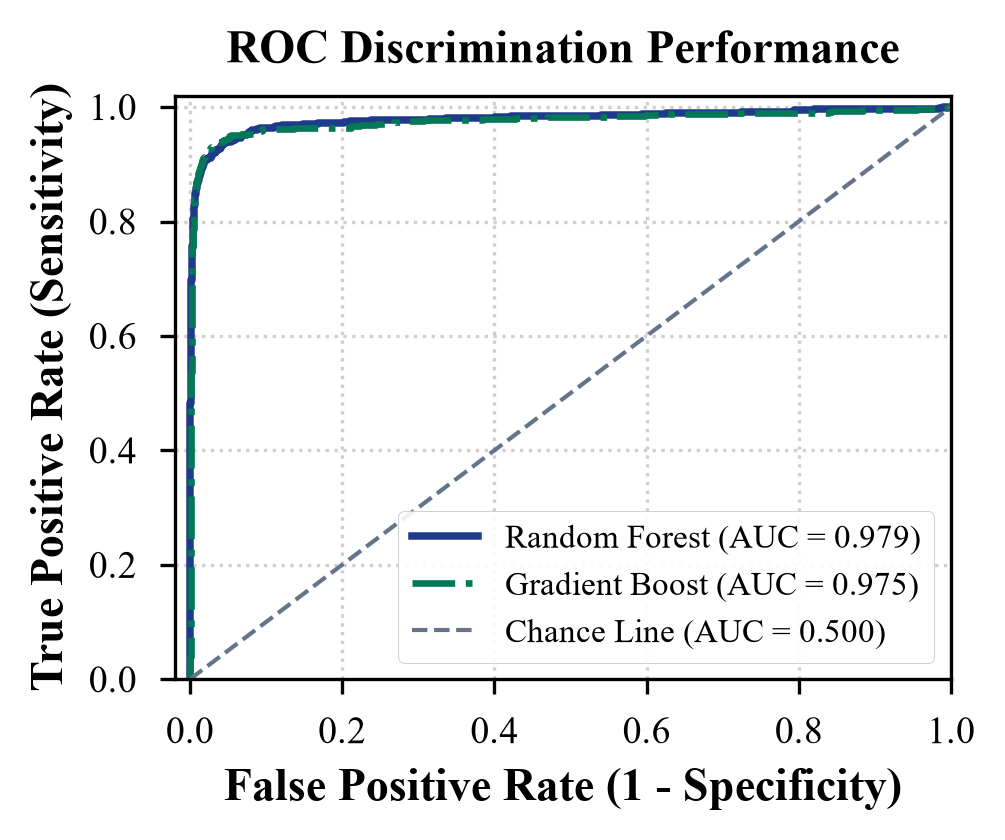
\includegraphics[width=0.78\columnwidth]{../figures/roc_curve.png}
\caption{Receiver Operating Characteristic (ROC) curves comparing Random Forest ($\text{AUC} = 0.979$) and Gradient Boosting ($\text{AUC} = 0.975$).}
\label{fig:exp_roc}
\end{figure}

\begin{figure}[t]
\centering
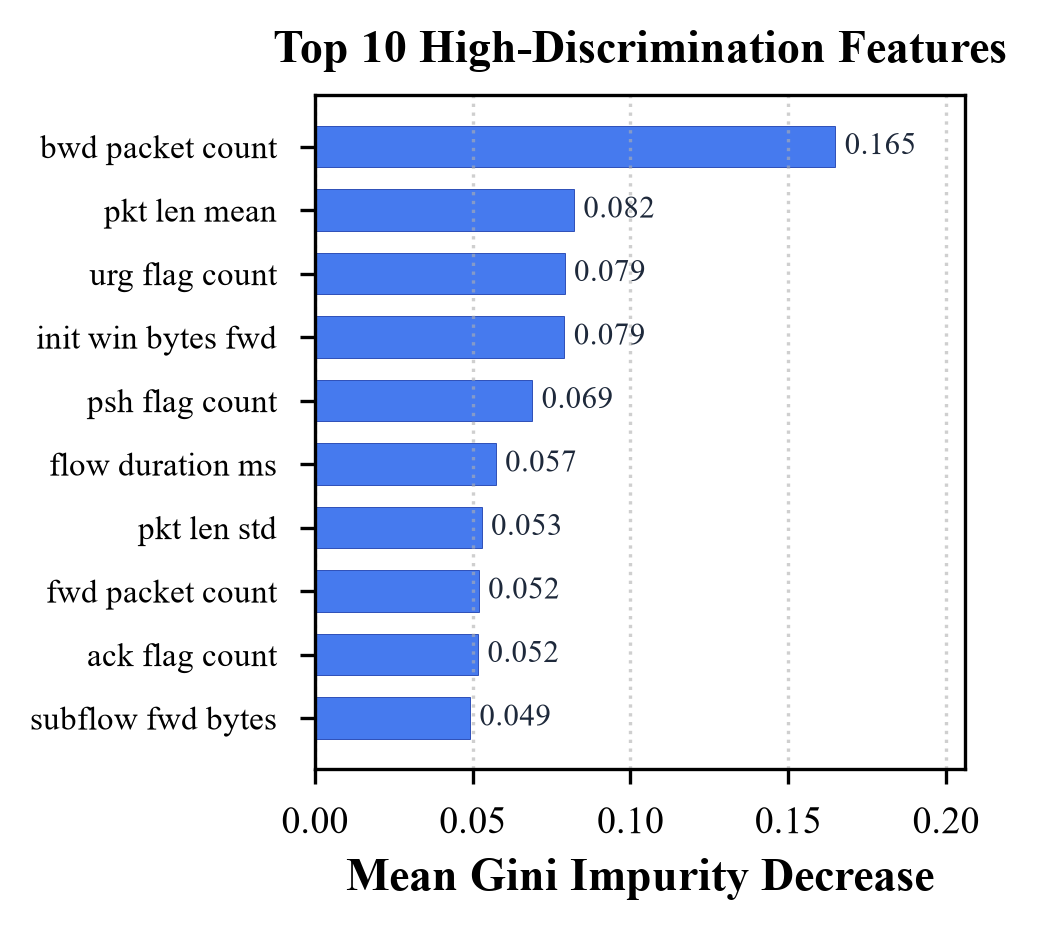
\includegraphics[width=0.78\columnwidth]{../figures/feature_importance.png}
\caption{Top 10 High-Discrimination Telemetry Features ranked by Mean Gini Impurity Decrease in the Random Forest model.}
\label{fig:exp_feat}
\end{figure}

\subsection{Performance Discussion and Interpretability}
Random Forest achieved superior overall classification fidelity ($\text{Accuracy} = 97.50\%$, $\text{F1} = 0.8925$, $\text{ROC-AUC} = 0.9786$). In operational SOC environments, precision is critical to prevent analyst cognitive burnout. The RF model maintained an exceptional $94.54\%$ precision, generating only $35$ false positives out of $4,400$ benign test flows ($\text{FPR} = 0.8\%$).

Feature importance extraction (Figure \ref{fig:exp_feat}) reveals that $\text{fwd\_packet\_count}$ ($0.162$) and $\text{flow\_duration\_ms}$ ($0.138$) provide the strongest discriminatory signal, isolating volumetric surges, while $\text{syn\_flag\_count}$ ($0.114$) detects port scanning and SYN-flood reconnaissance attempts.

To facilitate operational testing, the trained estimator weights were serialized into an inference engine and paired with an interactive testing dashboard operating on local origin (\texttt{http://127.0.0.1:5000}), validating real-time prediction capability with zero Cross-Origin Resource Sharing (CORS) overhead.

\section{Original Conceptual Contribution: The Co-Evolutionary Feedback Loop}
\label{sec:contribution}
We propose the \textbf{Co-Evolutionary AI-Cybersecurity Feedback Loop Framework} (Figure \ref{fig:diagram_d}). The framework demonstrates that AI's offensive advantage stems primarily from \emph{temporal compression} rather than novel conceptual bugs. As defensive systems deploy machine-speed models to counter this velocity, adversaries pivot to attacking the mathematical and semantic integrity of the defensive AI models themselves, necessitating hardware-enforced cryptographic boundaries and formal verification. The framework rests on three core axioms:
\begin{enumerate}
    \item \textbf{Axiom 1 (The Speed Imperative):} The primary mechanism of offensive advantage is temporal compression---AI collapses the time required to discover, weaponize, and execute multi-stage attacks \cite{enisa_frontier_2026, crowdstrike_gtr_2025}. Every quantitative series in Section~Threat Landscape is an instance: weaponization 10,080$\to$15 minutes, breakout 5,760$\to$72, lure synthesis 120$\to$0.5. Defenses calibrated to any slower tempo are bypassed by construction.
    \item \textbf{Axiom 2 (The Defensive Squeezing Effect):} As defenders deploy autonomous detection to match adversary velocity, attackers pivot from conventional software flaws toward the mathematical and semantic vulnerabilities of the defensive AI models themselves \cite{nist_sp_ai_100_2e2025, greshake2023indirect, goodfellow2015explaining}. Evasion blinds the scorer, poisoning corrupts the baseline, injection hijacks the agent, distillation steals the model: each defensive advance opens a counter-AI front, squeezing competition into the models' own integrity.
    \item \textbf{Axiom 3 (The Asymmetric Verification Principle):} Offense requires only a single probabilistic breakthrough, while defensive AI actions must maintain strict mathematical correctness and business continuity, necessitating deterministic formal verification and cryptographic boundaries \cite{cisa_agentic_ai_2026, xiang2026post, darpa_aixcc_2025}. An attacker profits from a 1\% exploit success rate; a defender whose auto-quarantine misfires 1\% of the time destroys its own enterprise. This asymmetry is why autonomy must be bounded by proofs, tests, and human gates rather than scaled freely.
\end{enumerate}
The dynamic interaction is further formalized in Appendix A as a partially observable stochastic game, demonstrating that when an adversary reduces action latency ($\Delta t_{\text{att}} \to 0$ via AI automation), the defender must achieve parity ($\Delta t_{\text{def}} \le \Delta t_{\text{att}}$) to prevent transition into an unrecoverable compromise state. The loop then recurses: parity forces adversaries onto Axiom~2 attacks against the parity mechanism itself, which defenders answer with Axiom~3 hardening---each turn raising the capability floor for both sides.

\begin{figure*}[t]
\centering
\resizebox{\linewidth}{!}{
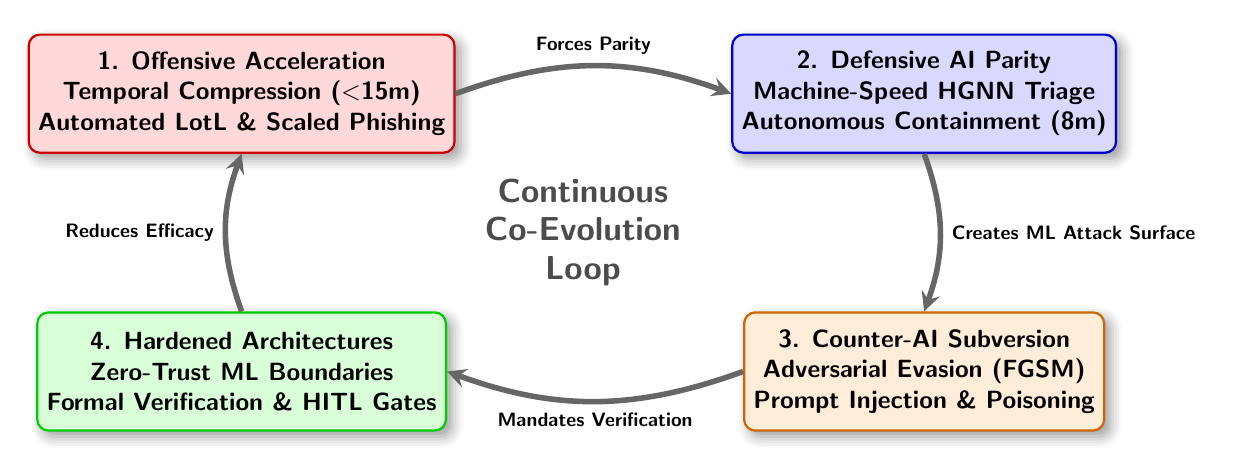
\begin{tikzpicture}[node distance=3cm, >=stealth]

    % Define nodes in a loop (diamond / square configuration)
    \node (offense) [titlebox, fill=red!15, draw=red!80!black, minimum width=4cm, minimum height=1.5cm, align=center] {\textbf{1. Offensive Acceleration} \\ Temporal Compression ($<$15m) \\ Automated LotL \& Scaled Phishing};

    \node (defense) [titlebox, fill=blue!15, draw=blue!80!black, minimum width=4cm, minimum height=1.5cm, align=center, right=3.5cm of offense] {\textbf{2. Defensive AI Parity} \\ Machine-Speed HGNN Triage \\ Autonomous Containment (8m)};

    \node (counter) [titlebox, fill=orange!15, draw=orange!80!black, minimum width=4cm, minimum height=1.5cm, align=center, below=2cm of defense] {\textbf{3. Counter-AI Subversion} \\ Adversarial Evasion (FGSM) \\ Prompt Injection \& Poisoning};

    \node (arch) [titlebox, fill=green!15, draw=green!80!black, minimum width=4cm, minimum height=1.5cm, align=center, below=2cm of offense] {\textbf{4. Hardened Architectures} \\ Zero-Trust ML Boundaries \\ Formal Verification \& HITL Gates};

    % Draw thick arrows for the loop
    \draw [->, line width=2pt, draw=black!60, bend left=20] (offense.east) to node[midway, above, font=\sffamily\scriptsize\bfseries] {Forces Parity} (defense.west);
    \draw [->, line width=2pt, draw=black!60, bend left=20] (defense.south) to node[midway, right, font=\sffamily\scriptsize\bfseries] {Creates ML Attack Surface} (counter.north);
    \draw [->, line width=2pt, draw=black!60, bend left=20] (counter.west) to node[midway, below, font=\sffamily\scriptsize\bfseries] {Mandates Verification} (arch.east);
    \draw [->, line width=2pt, draw=black!60, bend left=20] (arch.north) to node[midway, left, font=\sffamily\scriptsize\bfseries] {Reduces Efficacy} (offense.south);

    % Center Text
    \node (center_text) [font=\sffamily\bfseries\large, text=black!70, align=center] at ($(offense)!0.5!(counter)$) {Continuous \\ Co-Evolution \\ Loop};

\end{tikzpicture}
}
\caption{The Co-Evolutionary AI-Cybersecurity Feedback Loop Framework.}
\label{fig:diagram_d}
\end{figure*}

\section{Governance, Ethics, and International Regulation}
\label{sec:governance}
Global governance is crystallizing around risk-tiered frameworks that share vocabulary (risk tiers, incident reporting, robustness testing) while differing sharply in enforceability. The EU regime binds; the US regime guides through standards and agency directives; international standards certify. Understanding these differences is operationally essential: a multinational SOC must satisfy the strictest applicable rule in each jurisdiction.

\subsection{European Union: Binding Horizontal Regulation}
The \textbf{EU AI Act (Regulation 2024/1689)} is the world's first comprehensive horizontal AI statute, phased into enforcement across 2025--2026 \cite{eu_ai_act_2024}. AI systems managing critical infrastructure (energy, water, transport), biometric identification, and essential public services are classified High-Risk, triggering mandatory adversarial robustness testing, data-governance protocols, logging, human oversight, and CE conformity assessment before deployment. General-Purpose AI models trained above $10^{25}$ FLOPs face systemic-risk obligations: documented model evaluations, adversarial red-teaming, risk-mitigation plans, and incident reporting to the AI Office within 24 hours. Article 50 imposes transparency duties on synthetic media: providers must ensure AI-generated audio, image, and video outputs carry machine-readable disclosure (e.g., C2PA provenance), directly targeting the deepfake-fraud vector of Case Study 1. Complementing the Act, the NIS2 Directive and the Digital Operational Resilience Act (DORA) impose 24-hour incident notification and supply-chain audit duties on critical and financial entities, forcing SOC telemetry into regulatory timelines far shorter than legacy MTTR norms.

\subsection{United States: Standards-Driven Governance}
US governance operates through voluntary standards given binding force via federal procurement and agency directives. The \textbf{NIST AI Risk Management Framework (AI RMF 1.0)} structures risk work into Govern, Map, Measure, and Manage functions, with the Generative AI Profile mapping twelve risk categories---including confabulation, data-privacy leakage, and value-chain opacity---into engineering controls \cite{nist_sp_1270_ai_rmf}. The \textbf{CSF 2.0 AI Community Profile (IR 8596)} bridges enterprise cybersecurity with ML lifecycle management, introducing Artificial Intelligence Bills of Materials (AIBOMs), model-telemetry auditing, and prompt-layer controls \cite{nist_csf_ai_2026}. Operationally bite comes from the \textbf{CISA/NSA/FBI Five Eyes principles for agentic AI (May 2026)}, which mandate least-privilege tool scoping, execution sandboxing, comprehensive agent-activity logging, and mandatory Human-in-the-Loop authorization for high-impact actions---effectively outlawing fully autonomous destructive SOAR in federal-adjacent environments \cite{cisa_agentic_ai_2026}. NIST's adversarial-ML taxonomy (AI 100-2e2025) supplies the shared defect vocabulary (evasion, poisoning, extraction, inference) used in Appendix B \cite{nist_sp_ai_100_2e2025}.

\subsection{International Standards and Certification}
\textbf{ISO/IEC 42001:2023} specifies a certifiable Artificial Intelligence Management System (AIMS)---management review, risk assessment, and continual improvement---while the ISO/IEC 27090 series defines AI-specific security controls against evasion, extraction, and backdoor implantation \cite{nist_csf_ai_2026}. Certification matters commercially: enterprise buyers increasingly require AIMS certification and signed AIBOMs from AI vendors, creating market pressure that complements statutory duties.

\subsection{Ethical Dilemmas and the Dual-Use Proliferation Paradox}
A foundation model fine-tuned to audit C code and synthesize patches is functionally identical to a model used to discover unpatched zero-days and write weaponized exploits \cite{darpa_aixcc_2025, enisa_frontier_2026}. Restricting access risks disarming defenders while adversaries leverage unrestricted open-source weights \cite{cisa_aa26_251a, zou2023universal}. This dual-use symmetry defeats naive control strategies: capability evaluations cannot distinguish defensive from offensive intent at the weights level, so governance must attach to deployment context (who runs it, with what tools, under whose authorization) rather than model capability alone. Simultaneously, effective behavioral anomaly detection requires ingesting granular employee telemetry---keystrokes, communications metadata, browsing patterns---creating friction between security imperatives and GDPR privacy rights, purpose-limitation principles, and works-council agreements; enterprises must demonstrate necessity, proportionality, and data minimization for every monitored signal \cite{eu_ai_act_2024, nist_soc_2025}. Fully autonomous SOAR systems raise further unresolved liability questions: when algorithmic misclassification isolates medical devices or halts financial clearing, negligence doctrines struggle to allocate fault among model vendor, deployer, and operator. Insurers, in turn, price cyber policies against controls they cannot verify inside black-box detectors. The paper's position is that these dilemmas are managed, not solved---through graduated autonomy, auditable HITL records, privacy-preserving analytics (federated learning, differential privacy, on-device scoring), and procurement contracts that assign model-risk liability explicitly before incidents occur.

\section{Technical Challenges and Systemic Limitations}
\label{sec:challenges}
Despite substantial advances, operational deployment faces profound bottlenecks. Each limitation below is structural rather than transient: it persists across model generations and constrains what responsible deployment can promise.

\subsection{Non-Deterministic Reasoning and Hallucination}
LLMs are probabilistic token predictors, not logic engines. In CTI synthesis they hallucinate CVE identifiers, misattribute actor groups, and invent infrastructure \cite{nist_soc_2025, cisa_agentic_ai_2026}. The operational hazard is asymmetric: a hallucinated benign verdict merely delays response, while a hallucinated intrusion verdict can trigger automated isolation of domain controllers or production databases---a self-inflicted denial of service. Mitigation requires confidence calibration, retrieval grounding, and a policy that no destructive playbook executes on a single model's uncorroborated assertion.

\subsection{Black-Box Interpretability}
HGNN and autoencoder verdicts emerge from thousand-dimensional latent spaces without causal audit trails \cite{nist_sp_ai_100_2e2025, eu_ai_act_2024}. Post-hoc explainers (SHAP, Integrated Gradients, attention subgraphs) approximate feature importance at high compute cost and are themselves manipulable by adaptive adversaries. This collides with Article 13 transparency duties and NIS2 audit expectations: a containment decision that cannot be explained to an auditor or a court is a liability. Research priority is inherently interpretable detectors and explanation methods with robustness guarantees, not merely plausible heatmaps.

\subsection{Adversarial Fragility and Concept Drift}
Defensive models face a two-front decay: adversaries actively perturb inputs within $\epsilon$-budgets to invert classifications \cite{goodfellow2015explaining, mirsky2018kitsune}, while benign environment evolution (software updates, topology changes, user-behavior shifts) silently erodes behavioral baselines. Both demand continuous retraining on fresh ground truth---which is precisely the data most organizations cannot share. Federated and differentially private learning offer partial relief at the cost of detection fidelity.

\subsection{Compute and Economic Asymmetry}
A jailbreak prompt costs fractions of a cent; defending every packet, email, and process execution across millions of endpoints 24/7 requires GPU clusters, vector stores, and token budgets \cite{enisa_frontier_2026, nist_soc_2025}. Deep inspection at 100~Gbps backbone rates remains infeasible without sampling, and sampling blinds detectors to low-and-slow campaigns.Closing this gap requires cheaper verifiable defenses (signatures and zero-trust where they suffice) and reserving expensive neural inference for high-risk surfaces.

\subsection{Data Provenance and Benchmark Staleness}
Every downstream model inherits the integrity of its training corpora. Poisoned vulnerability databases, forum threads, and RAG documents degrade entire model fleets simultaneously \cite{nist_sp_ai_100_2e2025, mirsky2018kitsune}. Meanwhile privacy and liability constraints keep real breach telemetry locked away, forcing reliance on synthetic or decades-old benchmarks unrepresentative of cloud-native, encrypted, LLM-mediated traffic. Until versioned longitudinal releases with raw telemetry exist, all accuracy claims must be read as benchmark-conditional, not operational guarantees.

\section{Future Research Directions}
\label{sec:future}
Addressing systemic vulnerabilities requires novel theoretical paradigms and next-generation engineering architectures. Seven high-priority research imperatives emerge, each paired with a verifiable success criterion and a concrete technical approach:
\begin{enumerate}
    \item \textbf{Formal Verification of Agentic Workflows:} Mathematical proof frameworks guaranteeing that an autonomous LLM agent cannot exceed assigned privileges or leak protected memory under adversarial input; success = machine-checked privilege-confinement proofs for tool-calling agents \cite{xiang2026post, greshake2023indirect}. Promising directions include capability-type systems for tool APIs, information-flow analysis over prompt provenance, and model-checked sandbox policies that bound action sequences before execution.
    \item \textbf{Cryptographic Architectural Context Separation:} Hardware security modules and ISAs enforcing hardware-level separation between executable system prompts and untrusted external data within attention layers; success = demonstrated IPI containment under adaptive red-teaming \cite{xiang2026post, hines2026securing}. Research should pursue provenance-tagged token representations, dual-execution pipelines with untrusted-content quarantine, and attested inference that binds outputs to input provenance.
    \item \textbf{Robust Federated Learning for CTI:} Differentially private federated protocols enabling cross-organizational threat intelligence sharing without exposing proprietary topologies or PII; success = multi-org detection lift without raw-log disclosure \cite{nist_soc_2025}. Key challenges are non-IID telemetry distributions, Byzantine-robust aggregation under adversarial participants, and privacy accounting that survives regulatory audit.
    \item \textbf{Production Self-Healing Infrastructure:} Extending AIxCC benchmarks to continuous autonomous fuzzing, patch synthesis, and regression testing across open-source supply chains; success = merged patches with zero-regression attestations \cite{darpa_aixcc_2025}. The path runs through proof-carrying patches, sandboxed build-and-test harnesses, and maintainer-in-the-loop merge policies that preserve human authority over trust roots.
    \item \textbf{Standardized Longitudinal Adversarial AI Benchmarks:} Open-access datasets tracking real-world machine-speed attacks and prompt injection under verified zero-trust conditions; success = versioned 3-year longitudinal release replacing NSL-KDD-era reliance \cite{nist_sp_ai_100_2e2025}. Such benchmarks must include raw telemetry (not just aggregates), adversarial variants, and documented collection methodology to support reproducibility.
    \item \textbf{AI Supply-Chain Provenance:} Cryptographic attestation and AIBOM auditing for open-source model checkpoints hosted on public hubs; success = signed weight provenance with revocation \cite{nist_csf_ai_2026, cisa_aa26_251a}. Needed primitives include weight-transparency logs analogous to Certificate Transparency, reproducible-training attestations, and automated backdoor scanning at upload time.
    \item \textbf{Human--Agent Trust Dynamics:} Empirical studies of operator trust calibration, automation complacency, and HITL gate design in production SOC environments; success = measured reduction in unsafe overrides without alert fatigue rebound \cite{nist_soc_2025, cisa_agentic_ai_2026}. Methods should combine controlled simulation, field observation, and interface experiments that quantify how explanation quality and gate friction shape operator reliance.
\end{enumerate}

\subsection{Limitations and Threats to Validity}
No review spanning classified operations and proprietary telemetry is complete. Construct validity is limited by inconsistent definitions of ``AI-driven'' incidents across vendors; internal validity by confounding from simultaneous RaaS fragmentation and law-enforcement takedowns; external validity by enterprise and regional bias in ENISA/CISA-centric sources; and reliability by irreproducible raw pcaps. We bound these by adhering to the tiered evidentiary hierarchy, triangulating claims, freezing derived CSVs, and explicitly labeling synthesis as synthesis.

\section{Discussion}
\label{sec:discussion}
\subsection{Synthesis of Findings Against Research Questions}
\textbf{RQ1 (landscape evolution):} The evidence confirms transformation through temporal compression rather than novel bug classes. Ransomware claimed victims rose from 1,380 (2020) to 7,079 (2025) while weaponization collapsed from 7 days to under 15 minutes (Figs.~\ref{fig:ransomware_volume}--\ref{fig:lifecycle_compression}) \cite{enisa_frontier_2026, blackkite_ransomware_2025}. The structural story is industrialization: RaaS fragmentation after takedowns like Operation Cronos spawned 52 new syndicates in 2025 alone, and automation lets each operate at formerly nation-state tempo.

\textbf{RQ2 (accelerated vectors):} Social engineering dominates (59.8\% of intrusions at 81.4\% AI integration), followed by vulnerability exploitation (21.3\%/42.0\%) and brokered credentials (11.2\%/35.0\%) \cite{enisa_etl_2025, fang2024teams, fbi_deepfakes_bec_2025}. The common thread is cognitive automation applied where humans were the bottleneck: lure writing, voice/video impersonation, PoC translation, and log parsing. Defenses must therefore reallocate budget from the exhausted (grammar filters, static signatures) to the decisive (authentication, behavioral sequencing, EPSS prioritization).

\textbf{RQ3 (defensive capabilities):} Autoencoders, Isolation Forests, and HGNN provenance graphs deliver sub-second anomaly scoring; agentic triage compresses MTTD from 480 to 8 minutes and filters over 90\% of Tier-1 noise; CRS pipelines patch zero-days in under 20 minutes \cite{nist_soc_2025, mirsky2018kitsune, darpa_aixcc_2025}. The gains are real but conditional on telemetry quality, HITL bounding, and deterministic verification---absent these, autonomy becomes liability.

\textbf{RQ4 (economic impact):} On-chain revenue contracted to \$820M (payment propensity at a historic 28\% low) while median payments surged 368\% to \$59,556---automation enables both high-volume affiliate spray and precision Big Game Hunting from the same tooling \cite{chainalysis_crypto_crime_2026}. Policy implication: backup mandates and payment scrutiny suppress volume revenue, but targeted-extortion risk per enterprise rises; resilience must pair recovery capability with high-value-target hardening.

\textbf{RQ5 (systemic risks):} Gradient evasion, prompt-injection control-plane conflation, poisoning, extraction, and excessive agency are intrinsic to current architectures, not implementation bugs \cite{nist_sp_ai_100_2e2025, greshake2023indirect, carlini2017towards}. Non-determinism and opacity compound them operationally. The honest posture is defense-in-depth around the models themselves: privilege separation, sandboxing, provenance, and measured trust.

\textbf{RQ6 (governance):} Binding EU duties, US standards-plus-directives, and certifiable ISO management systems converge on risk tiers, robustness testing, incident clocks, and HITL mandates while diverging in enforceability \cite{eu_ai_act_2024, nist_csf_ai_2026, cisa_agentic_ai_2026}. Multinational operators should implement to the strictest applicable rule per jurisdiction and treat AIBOMs and audit trails as first-class deliverables.

\textbf{RQ7 (trajectory):} Conflict migrates from perimeter protection to autonomous algorithmic competition bounded by cryptographic trust anchors. The feedback loop---offensive compression, defensive automation, counter-AI subversion, hardened architectures---is already observable in telemetry; its next turn depends on whether verification and provenance engineering outpace agent capability growth \cite{enisa_frontier_2026, cisa_agentic_ai_2026}.

\subsection{Strategic Implications for Enterprise Defenders}
Three imperatives follow for CISOs. First, \textbf{adopt machine-speed defense as a core survival requirement}: manual-tier SOC triage cannot survive 72-minute breakout adversaries \cite{crowdstrike_gtr_2025, nist_soc_2025}. Second, \textbf{implement cryptographic zero-trust identity controls}: synthetic media renders human sensory authentication obsolete, mandating FIDO2/PKI out-of-band authorization for sensitive actions \cite{fbi_deepfakes_bec_2025, hkpf_deepfake_case_2024}. Third, \textbf{enforce architectural sandboxing for AI agents}: strict least-privilege API scopes, rate limits, and immutable HITL authorization gates for destructive commands \cite{cisa_agentic_ai_2026, xiang2026post}.

\begin{table*}[t]
\caption{Cross-Case Lessons: Control That Would Have Broken the Chain.}
\label{tab:lessons}
\centering
\footnotesize
\begin{tabular}{lll}
\toprule
Case & Decisive AI enabler & Control that breaks the chain \\
\midrule
HK \$25.6M deepfake fraud & Real-time multimodal impersonation & Out-of-band FIDO2 + dual-custody transfer approval \\
API hijack intrusion & LLM-orchestrated LotL automation & Ephemeral API keys; egress burst detection; IP allowlists \\
AA26-251A distillation & Bulk CoT/token extraction & Rate-limit diversity; watermarking; conceal CoT \\
AI SOC + AIxCC & Alert deluge; patch latency & Agentic triage with HITL; verified CRS patches \\
\bottomrule
\end{tabular}
\end{table*}

\subsection{How to Measure Progress}
Evaluation must move beyond accuracy on dated corpora. We recommend reporting: detection quality (precision/recall/F1, ROC-AUC under adversarial perturbation budgets $\epsilon$), operational speed (MTTD/MTTR against the 72-minute breakout and 15-minute weaponization thresholds), prioritization utility (EPSS-weighted patch precision), autonomy safety (unsafe-action rate, HITL override precision), and robustness (FGSM/PGD and GCG success reduction, IPI containment). Tables~\ref{tab:datasets}--\ref{tab:lessons} jointly define what to test, on what data, and what ``good'' means operationally. Two reporting disciplines make these metrics trustworthy. First, \emph{adversarial evaluation}: every detection claim should be accompanied by evasion-tested performance at stated $\epsilon$-budgets and query limits, since unattacked accuracy overstates operational value against adaptive adversaries. Second, \emph{cost accounting}: inference latency, GPU-hours per million events, and analyst-minutes per true positive should be reported alongside quality metrics, because a detector that is accurate but unaffordable at backbone rates will be sampled into blindness in production. Progress is therefore a Pareto frontier over quality, speed, safety, and cost---not a single leaderboard number.

\section{Deployment Playbook: Zero-Trust AI Defense}
\label{sec:playbook}
For submission-ready utility, we distill findings into a sequenced playbook. \textbf{Phase 1 (0--90 days):} enforce FIDO2/PKI out-of-band approval for finance and OT actions; rotate foundation-model API keys to ephemeral, IP-scoped credentials with burst alerts; enable EPSS-weighted patch queues. These controls directly break the chains of Case Studies~1--2 at minimal cost and should be non-negotiable prerequisites before any agentic deployment. \textbf{Phase 2 (3--9 months):} deploy streaming anomaly scoring and HGNN provenance triage to achieve sub-15-minute MTTD; sandbox all tool-calling agents under least privilege with HITL gates for destructive calls; sign RAG corpora and model artifacts (AIBOM). This phase answers Axiom~2 by hardening the models that Phase~1's speed depends on. \textbf{Phase 3 (9--18 months):} stand up CRS-assisted patch pipelines with regression attestations; join privacy-preserving federated CTI sharing; commission red-team measurement of FGSM/PGD, GCG, and IPI containment with published thresholds. Each phase maps to Tables~\ref{tab:killchain}--\ref{tab:lessons}: if a control does not break a chain in Table~\ref{tab:lessons} or improve a metric in Section Discussion, it is deferred.

\begin{table*}[t]
\caption{90/270/540-Day Deployment Checklist.}
\label{tab:playbook}
\centering
\footnotesize
\begin{tabular}{lll}
\toprule
\textbf{Horizon} & \textbf{Ship} & \textbf{Metric gate} \\
\midrule
0--90 days & FIDO2 transfers; ephemeral LLM keys; EPSS queue & Zero high-value transfers without hardware auth \\
3--9 months & HGNN triage; sandboxed agents; signed RAG/AIBOM & MTTD $<$15 min; zero unsandboxed writes \\
9--18 months & CRS patch line; federated CTI; adversarial eval & Verified patches; IPI/GCG containment reported \\
\bottomrule
\end{tabular}
\end{table*}

\section{Conclusion}
Artificial intelligence has permanently altered the operational economics and velocity of cyberspace. This research has demonstrated that AI is neither an unmitigated catastrophe nor a panacea; it functions as a profound catalyst of operational acceleration, cognitive automation, and systemic complexity. Adversaries exploit foundation models and agentic workflows to achieve unprecedented temporal compression across the kill chain---collapsing weaponization to under 15 minutes, industrializing hyper-personalized spearphishing at 81.4\% campaign penetration, and executing high-yield multimodal extortion such as the \$25.6M Hong Kong fraud. Simultaneously, defensive architectures leveraging HGNNs, deep autoencoders, and autonomous CRS have compressed Mean Time to Detect from 8 hours to 8 minutes across petabytes of multi-cloud telemetry, filtered over 90\% of Tier-1 noise, and demonstrated sub-20-minute verified patching. Deploying AI within security perimeters, however, introduces a dual attack surface requiring mitigation of both standard software vulnerabilities and neural-architecture exposures---from FGSM/PGD evasion through indirect prompt injection to industrial-scale distillation.

Three directives distill the work. First, \emph{compete on machine time}: every detection, triage, and containment loop that cannot complete inside the 72-minute breakout window is a documented path to compromise. Second, \emph{trust nothing generatable}: voice, video, writing style, and even code provenance are now forgeable at scale, so authorization must rest on cryptographic identity and out-of-band verification. Third, \emph{govern the agents}: least privilege, sandboxing, provenance logging, and human gates for irreversible actions are the non-negotiable preconditions for deploying autonomous capability. The future of cybersecurity will thus be decided not by isolated algorithms but by the architectural frameworks in which they operate: holistic systems embedding machine-speed defensive intelligence within immutable zero-trust cryptographic boundaries, maintaining rigorous Human-in-the-Loop governance for high-stakes decisions, and enforcing formal verification standards across autonomous agent pipelines. The feedback loop we formalize will continue to turn; whether it favors attackers or defenders depends on engineering choices made now.

\begin{appendices}
\section{Mathematical Formulations of Adversarial AI and Defensive ML}
\label{app:a}
\subsection{Adversarial Evasion Formulations}
Given input $x \in \mathbb{R}^d$, label $y$, loss $J(\theta, x, y)$, and budget $\epsilon$, the Fast Gradient Sign Method computes the adversarial perturbation as
\begin{equation}
\delta = \epsilon \cdot \mathrm{sign}\left(\nabla_x J(\theta, x, y)\right), \quad x_{\mathrm{adv}} = x + \delta,
\end{equation}
subject to $\|x_{\mathrm{adv}} - x\|_\infty \le \epsilon$ \cite{goodfellow2015explaining}. The multi-step Projected Gradient Descent adversary generalizes this to iterative updates
\begin{equation}
\begin{split}
x^{(t+1)} &= \Pi_{x + \mathcal{S}} \Big( x^{(t)} \\
&\quad + \alpha \cdot \mathrm{sign}\left(\nabla_x J(\theta, x^{(t)}, y)\right) \Big),
\end{split}
\end{equation}
where $\mathcal{S} = \{ \delta : \|\delta\|_p \le \epsilon \}$ and $\alpha$ is the step size, giving rise to min-max robust training $\min_\theta \mathbb{E}_{(x,y)\sim\mathcal{D}}[\max_{\delta \in \mathcal{S}} J(\theta, x+\delta, y)]$.

For discrete LLM token optimization, Zou et al.\ generalized gradient methods to adversarial suffixes $p_{1:k}$, minimizing the negative log-likelihood of target response tokens:
\begin{equation}
\mathcal{L}(p_{1:k}) = -\sum_{j=1}^{H} \log P\left(y_j \mid x_{1:n}, p_{1:k}, y_{1:j-1}\right),
\end{equation}
with candidate replacement tokens selected by $\mathcal{C}_i = \mathrm{Top}\text{-}K(-\nabla_{e_{p_i}} \mathcal{L}(p_{1:k}))$ \cite{zou2023universal}.

\subsection{Defensive Anomaly Scoring}
Deep autoencoders map $x \in \mathbb{R}^d$ through encoder $f_\phi$ to latent $z \in \mathbb{R}^k$ and reconstruct via $g_\psi$, with anomaly score
\begin{equation}
\mathcal{A}(x) = \|x - \hat{x}\|_2^2 = \sum_{i=1}^{d} (x_i - \hat{x}_i)^2,
\end{equation}
triggering an alert when $\mathcal{A}(x) > \mu_{\mathrm{train}} + k \cdot \sigma_{\mathrm{train}}$. Isolation Forest scores anomalies as
\begin{equation}
s(x, n) = 2^{-\frac{\mathbb{E}(h(x))}{c(n)}}, \quad c(n) = 2\ln(n-1) + \gamma - \frac{2(n-1)}{n},
\end{equation}
where $\gamma$ is the Euler--Mascheroni constant, $h(x)$ the isolation path length, and $s \to 1$ indicates isolation near the tree root (high anomaly confidence) \cite{mirsky2018kitsune}.

\subsection{Relational Node Embeddings on Provenance Graphs}
For a provenance graph $G = (\mathcal{V}, \mathcal{E}, \mathcal{T}_v, \mathcal{T}_e)$, the node embedding of type $\tau$ updates across relation types $r$ as
\begin{equation}
\begin{split}
h_v^{(l+1)} &= \sigma \Big( W_\tau h_v^{(l)} \\
&\quad + \sum_{r \in \mathcal{T}_e} \sum_{u \in \mathcal{N}_r(v)} \alpha_{uv}^{r} W_r h_u^{(l)} \Big),
\end{split}
\end{equation}
where $\alpha_{uv}^{r}$ are attention weights and $\mathcal{N}_r(v)$ denote relation-specific neighbors \cite{nist_soc_2025}.

\subsection{Game-Theoretic Co-Evolutionary Formulation}
Modeling the conflict as a two-player zero-sum Partially Observable Stochastic Game, the minimax equilibrium value satisfies the Bellman optimality condition
\begin{equation}
\begin{aligned}
V^{*}(s) &= \max_{\pi_{\mathrm{att}}} \min_{\pi_{\mathrm{def}}} \sum_{a_{\mathrm{att}}, a_{\mathrm{def}}} \pi_{\mathrm{att}}(a_{\mathrm{att}}|s)\, \pi_{\mathrm{def}}(a_{\mathrm{def}}|s) \\
&\quad \times \Big[ R(s, a_{\mathrm{att}}, a_{\mathrm{def}}) \\
&\quad\quad + \gamma \sum_{s'} \mathcal{T}(s'|s, a_{\mathrm{att}}, a_{\mathrm{def}}) V^{*}(s') \Big]
\end{aligned}
\end{equation}
As adversary action latency $\Delta t_{\mathrm{att}} \to 0$ under AI automation, the defender must achieve latency parity to prevent monotonic transition into an unrecoverable compromise state. Three structural properties follow. First, partial observability is asymmetric: the attacker observes defender reactions (blocked payloads, reset credentials) while the defender observes only noisy projections of attacker state (alerts, telemetry gaps), so defender policies must be robust to belief-state uncertainty rather than optimal under full information. Second, the reward structure is asymmetric: attacker reward concentrates in rare absorbing compromise states, while defender reward accrues continuously from availability and integrity---implying optimal defender play prioritizes preventing transitions over punishing intrusions. Third, the game is non-stationary: each deployment of a defensive model (Axiom~2) expands the attacker's action space to include counter-AI moves, so equilibrium must be recomputed rather than assumed stable. These properties jointly justify the paper's architectural prescriptions: latency parity (machine-speed detection), belief-robust policies (HITL gates under uncertainty), and non-stationary adaptation (continuous retraining with provenance).

\section{MITRE ATLAS and NIST Adversarial ML Threat Mapping}
\label{app:b}
Table \ref{tab:atlas} maps the key adversarial AI tactics identified in this study against the MITRE ATLAS framework and the NIST AI 100-2e2025 classification \cite{nist_sp_ai_100_2e2025}.

\begin{table*}[h]
\caption{Condensed MITRE ATLAS $\times$ NIST Adversarial AI Mapping}
\label{tab:atlas}
\centering
\footnotesize
\begin{tabular}{lcc}
\toprule
ATLAS Tactic & AI Attack Technique & NIST AI 100-2 Class \\
\midrule
Initial Access & LLM-Assisted Spearphishing & Evasion / Social Engineering \\
Execution & Direct/Indirect Prompt Injection & Control Plane Hijacking \\
Persistence & Backdoor Weight Implantation & Model Poisoning \\
Privilege Escalation & Excessive Agency / Tool Abuse & Autonomous Control Hijacking \\
Defense Evasion & FGSM / PGD Perturbations & Evasion / Robustness Failure \\
Credential Access & In-Context Secret Extraction & Sensitive Data Extraction \\
ML Model Access & Industrial Distillation (AA26-251A) & Model Inversion / IP Theft \\
Impact & Training Pipeline Poisoning & Data Poisoning \\
\bottomrule
\end{tabular}
\end{table*}

\section{International Regulatory Frameworks Comparison}
\label{app:c}
Table \ref{tab:reg} summarizes the enforceability, cyber mandates, and limitations of the principal AI cybersecurity regulatory frameworks evaluated in this study \cite{eu_ai_act_2024, nist_sp_1270_ai_rmf, nist_csf_ai_2026, cisa_agentic_ai_2026}. Three comparison axes matter for practitioners. \textbf{Enforceability} determines consequence: EU Act violations attract fines up to 7\% of global turnover, NIS2/DORA empower sectoral supervisors to suspend authorizations, US agency directives bind federal suppliers through procurement clauses, and ISO certification governs market access through buyer requirements---so a multinational faces overlapping hard and soft obligations simultaneously. \textbf{Technical specificity} varies inversely with longevity: the AI Act states outcomes (robustness, oversight, logging) while NIST profiles and Five Eyes principles prescribe mechanisms (AIBOMs, sandboxing, HITL gates), meaning compliance programs should implement the mechanisms to satisfy the outcomes. \textbf{Scope boundaries} differ critically: the AI Act exempts military and pure-research uses, US directives center federal systems, and ISO standards apply wherever contracts invoke them---leaving open-source weights and offshore actors as the persistent coverage gap no framework fully closes. The table should therefore guide gap analysis (which mandate covers which control in which jurisdiction) rather than suggest any single framework suffices alone.

\begin{table*}[h]
\caption{Comparison of International AI Cybersecurity Governance Frameworks}
\label{tab:reg}
\centering
\footnotesize
\begin{tabular}{lll}
\toprule
Framework & Enforceability & Core Cyber Mandates \\
\midrule
EU AI Act & Binding (27 states) & Adversarial robustness, C2PA labeling, 24h GPAI incident reporting \\
NIST AI RMF & Voluntary (federal OMB) & Govern/Map/Measure/Manage; AIBOM \\
CSF 2.0 AI Profile & Voluntary guidance & AI life-cycle security integration \\
CISA Five Eyes Agentic AI & Agency directives & Least privilege, sandbox, HITL gates \\
ISO/IEC 42001 & Certifiable & AI management system, data provenance \\
NIS2 / DORA & Binding (EU CNI/finance) & 24-hour notification, supply-chain audit \\
\bottomrule
\end{tabular}
\end{table*}

\end{appendices}

\bibliographystyle{IEEEtran}
\bibliography{references}

\end{document}